%% Template para TCC na classe IFBATCC
%% versao 1.0
%% (c) 2021 Antônio Cleber de Sousa Araújo
%% https://github.com/cleberaraujo/ifbatcc.git
%% versao 1.1
%% (c) 2023 Leandro Costa Souza
%% https://github.com/ifbasaj/tcc-template.git

%% Carrega a classe ifbatcc
%% Opcoes: * Idiomas
%%           pt   - português (padrao)
%%           en   - inglês
%%         * Tipos de Trabalhos (pelos graus de formação)
%%           tec  - para TCC de cursos tecnólogos (padrão)
%%           bsc  - para monografias de graduação
%%           msc  - para dissertações de mestrado
%%           qual - exame de qualificação de mestrado
%%           prop - exame de qualificação de doutorado
%%           phd  - para teses de doutorado
%%         * Cursos do IFBA/SAJ
%%           ads  - Análise e Desenvolvimento de Sistemas
%%           rde  - Redes de Computadores (padrão)
%%           mul  - Produção Multimídia
%%         * Mídia
%%           scr  - para versão eletrônica (PDF) / consulte o guia do usuário
%%         * Estilo
%%           classic - estilo original a la TAOCP (deprecated)
%%           std     - novo estilo a la CUP (padrão)
%%         * Paginação
%%           oneside - para impressão em face única
%%           twoside - para impressão em frente e verso (padrão)
\documentclass[tec, ads, scr, classic, a4paper, twoside]{ifbatcc}
\usepackage[utf8]{inputenc}
\usepackage{chngcntr}
\usepackage{float}

\usepackage{placeins}
\usepackage{adjustbox} % no preâmbulo
\usepackage{minted}
\usepackage{nomencl}
\makenomenclature

\renewcommand{\nomname}{\listabbreviationsname}
\renewcommand{\nomlabel}[1]{\textbf{#1}\hfil}

% Ajuste das cores de hyperlinks (remove vermelho/verde padrão do hyperref)
\AtBeginDocument{\hypersetup{hidelinks}}


%% Preâmbulo:
%% coloque aqui o seu preambulo LaTeX, i.e., declaração de pacotes,
%% (re)definicoes de macros, medidas, etc.

%% Identificação:

% Nome da biblioteca - usado na ficha catalográfica
% default: Biblioteca do IFBA Campus Santo Antônio de Jesus
\library{Biblioteca do IFBA \textit{Campus} Santo Antônio de Jesus}

% Programas de pós graduação
% e.g. \program{Pós graduação em Redes Linux}
%\program{Curso Superior em Tecnologia}

% Titulo do TCC
% e.g. \title{Redes de Computadores em SAJ}
\title{Aplicação de Modelos de Linguagem de Larga Escala (LLMs) na Verificação Automatizada da Conformidade entre Requisitos de Software e Código-Fonte}

% Data da defesa
% e.g. \date{19 de fevereiro de 2021}
\date{DATA DA DEFESA}

% Autor
% e.g. \author{José da Silva}
\author{Kaio Sande Tavares}

% Orientador(a)
% Opcao: [f] - para orientadora do sexo feminino
% e.g. \adviser[f]{Profa. Dra. Maria Santos}
\adviser{Leandro Costa Souza}

%% Inicio do documento
\begin{document}

%% Catalogação do TCC
%% IFBA/SAJ - Sigla do curso - Número ordinal de trabalhos dete curso
\ifbafrontpage{IFBA/SAJ-ADS-XXXX}

%%
%% Parte pre-textual
%%
\frontmatter

\ifbapresentationpage
% Se seu trabalho for uma dissertação de mestrado, use a linha acima
%\presentationpage
% Se for qualificação, use \presentationpage

% Ficha catalográfica
\authorcitationname{Tavares, Kaio Sande} % e.g. Sobrenome, Nome e sobrenome do meio
\advisercitationname{Souza, Leandro Costa} % e.g. Araújo, Antônio Cleber de Sousa
% \coadvisercitationname{NOME DO SEU CO-ORIENTADOR EM CITACOES} % e.g. Silva, João Santos
\catalogtype{TIPO DE TRABALHO} % e.g. ``Tese (doutorado)''
\catalogtopics{TOPICOS PARA FICHA CATALOGRAFICA} % e.g. ``1. Complexidade Estrutural. 2. Engenharia de Software''
\catalogcdd{NUMERO CDD} % e.g. ``CDD 20.ed. XXX.YY'' (esse número será passado pela biblioteca)
\catalogingsheet

%% Termo de aprovação
%% Composição da Banca Avaliadora
\approvalsheet{Santo Antônio de Jesus - BA, 05 de setembro de 2025}{
  \comittemember{Prof. Me. Leandro Costa Souza (Orientador)}{Instituto Federal da Bahia}
  \comittemember{Prof. Me. José Carlos Couto Souza Júnior}{Instituto Federal da Bahia}
  \comittemember{Prof. Caio Henrique Nascimento Valverde de Carvalho}{Instituto Federal da Bahia}
}

% Dedicatória
% Comente para ocultar
% \begin{dedicatory}
% DIGITE A DEDICATÓRIA AQUI
% \end{dedicatory}

% Agradecimentos
% Se preferir, crie um arquivo a parte e o inclua via \include{}
\acknowledgements

Agradeço primeiramente a Deus por ter me agraciado até aqui nesse momento, aos meus pais e meu irmão que sempre me deram apoio e suporte em todas as decisões, a minha avó Margarida e a minha dinda Lindy, que durante essa trajetória têm me acolhido e estado ao meu lado.

Em especial, eu quero agradecer ao primo e amigo Danilo por todas as conversas e oportunidades. Gratidão imensa! Ele tem extrema relevância na minha trajetória como estudante e profissional. Gratidão também à minha namorada Raquel, que está ao meu lado em todos esses anos e tem muita importância na minha vida; aos meus amigos, pelas conversas, companhia e todos os momentos — em especial à Tauynd, a qual nesses últimos anos foi uma irmã que a vida me deu.

Por fim, quero agradecer ao meu orientador Leandro e ao meu amigo Duda, os quais têm sido uma referência profissional para mim, por suas trajetórias, conhecimento e todos os momentos de debate e aprendizado que tive com eles.

\begin{flushright}
Obrigado a todos!
\end{flushright}

% Epigrafe
% Comente para ocultar
% e.g.
%  \begin{epigraph}[Tarde, 1919]{Olavo Bilac}
%  última flor do Lácio, inculta e bela,\\
%  És, a um tempo, esplendor e sepultura;\\
%  Ouro nativo, que, na ganga impura,\\
%  A bruta mina entre os cascalhos vela.
%  \end{epigraph}
% \begin{epigraph}[NOTA]{AUTOR}
% DIGITE AQUI A CITACAO
% \end{epigraph}

% Resumo em Portugues
% Se preferir, crie um arquivo separado e o inclua via \include{}
\resumo
Este trabalho investiga a aplicação de Modelos de Linguagem de Larga Escala (LLMs) como suporte à verificação automatizada da conformidade entre requisitos de software e sua implementação no código-fonte. Parte-se do reconhecimento de que a rastreabilidade entre especificações e artefatos de software é uma atividade essencial, porém propensa a falhas, omissões e retrabalho quando executada manualmente. Para tanto, são explorados fundamentos como vetorização semântica, janelas de contexto, engenharia de prompts e princípios de aprendizado de máquina aplicados ao domínio da engenharia de software.

A proposta foi validada por meio da análise de um sistema real, considerando dois módulos: um centrado em \textit{backend} e outro que envolve integração entre \textit{backend} e \textit{frontend}. Foram desenvolvidos prompts de auditoria capazes de orientar os modelos na inspeção automatizada dos arquivos do repositório, avaliando a presença ou ausência de implementações condizentes com os requisitos especificados. As saídas geradas pelos LLMs foram confrontadas com avaliações humanas e analisadas segundo métricas como acurácia simples, acurácia estrita, taxa de omissão, precisão, recall e f1-score.

Os resultados indicaram desempenho expressivo dos modelos, com acurácia estrita superior a 90\% em determinados cenários, evidenciando a viabilidade da abordagem como apoio à análise de conformidade. Apesar dos avanços, a solução apresenta limitações, como a dependência da janela de contexto e a necessidade de seleção criteriosa dos arquivos inspecionados. Como trabalho futuro, propõe-se a integração com agentes autônomos baseados no protocolo MCP, visando à automatização de ações corretivas, bem como a adoção de técnicas de recuperação aumentada por geração (RAG) para mitigar restrições impostas por repositórios extensos.

% Palavras-chave do resumo em Portugues
\begin{keywords}
LLM; Engenharia de Requisitos; Verificação Automatizada; Engenharia de Prompt
\end{keywords}

% Resumo em Inglês
% Se preferir, crie um arquivo separado e o inclua via \include{}
\abstract
This study investigates the application of Large Language Models (LLMs) as a support tool for the automated verification of compliance between software requirements and their implementation in source code. It is based on the recognition that traceability between specifications and software artifacts is a critical activity, yet prone to failures, omissions, and rework when performed manually. To address this, the study explores foundational concepts such as semantic vectorization, context windows, prompt engineering, and machine learning principles applied to the domain of software engineering.

The proposed approach was validated through the analysis of a real system, focusing on two modules: one primarily involving backend operations and another integrating backend and frontend components. Audit prompts were designed to guide the models in the automated inspection of repository files, evaluating the presence or absence of implementations consistent with the specified requirements. The outputs generated by the LLMs were compared to human evaluations and analyzed using metrics such as simple accuracy, strict accuracy, omission rate, precision, recall, and F1-score.

The results demonstrated significant performance by the models, with strict accuracy exceeding 90\% in certain scenarios, highlighting the feasibility of the approach as a support mechanism for compliance analysis. Despite these advances, the solution still presents limitations, such as context window constraints and the need for careful curation of the analyzed files. Future work includes integration with autonomous agents based on the MCP protocol to automate corrective actions, as well as the adoption of Retrieval-Augmented Generation (RAG) techniques to overcome limitations imposed by large code repositories.


\begin{keywords}
LLM; Requirements Engineering; Automated Verification; Prompt Engineering
\end{keywords}

% Sumario
% Comente para ocultar
\tableofcontents

% Lista de figuras
% Comente para ocultar
\listoffigures

% Lista de tabelas
% Comente para ocultar
\listoftables

% Lista de abreviaturas / nomenclatura
\printnomenclature[3cm]

%%
%% Parte textual
%%
\mainmatter
\counterwithout{figure}{chapter}
\counterwithout{table}{chapter}
\renewcommand{\thefigure}{\arabic{figure}}
\renewcommand{\thetable}{\arabic{table}}

% Recomendados criar cada capitulo em um arquivo separado, por exemplo
% "capitulo1.tex", "capitulo2.tex", ... "capituloN.tex" e depois
% inclui-los com:
% \include{capitulo1}
% \include{capitulo2}
% ...
% \include{capituloN}
%
% Importante: Use \xchapter ao invés de \chapter, conforme exemplo abaixo.
%\xchapter{Introdução}{Este é o primeiro capítulo, no qual eu conto toda a história deste trabalho.}


% ----------------------------------------------------------
\xchapter{Introdução}{}
\label{cap:introducao}
% ----------------------------------------------------------

A verificação da conformidade entre os requisitos de software e sua implementação constitui um desafio persistente na Engenharia de Software (ES), sobretudo em organizações que buscam entregar sistemas com agilidade, sem comprometer a qualidade. A crescente pressão por entregas rápidas, aliada à complexidade dos sistemas modernos, tem imposto uma sobrecarga significativa às equipes de qualidade, responsáveis por assegurar que as funcionalidades entregues estejam em consonância com as especificações previamente definidas. Esse cenário torna-se ainda mais crítico em projetos com alta rotatividade de desenvolvedores ou com documentação deficiente, nos quais a rastreabilidade entre o que foi solicitado e o que foi efetivamente entregue tende a se perder ao longo do ciclo de desenvolvimento.

Nesse contexto, o retrabalho torna-se uma consequência frequente, uma vez que a detecção precoce de falhas nem sempre é plenamente alcançada, o que compromete a confiabilidade e a sustentabilidade do produto. Para mitigar tais desafios, é comum que desenvolvedores e equipes de software utilizem ferramentas que contribuam para otimizar e agilizar suas atividades. Estratégias como testes automatizados, linters e analisadores estáticos de código desempenham papel relevante nesse cenário. No entanto, tais abordagens tendem a se concentrar predominantemente em aspectos técnicos e sintáticos do código-fonte, sendo, por vezes, insuficientes para avaliar a aderência funcional da implementação às regras de negócio previamente estabelecidas, sobretudo no que diz respeito às boas práticas e ao contexto dos requisitos.

Diante disso, propõe-se o uso de Large Language Models (LLMs) como ferramenta auxiliar na análise de conformidade entre requisitos e implementação, ainda durante a etapa de desenvolvimento. A ideia central consiste em empregar modelos de linguagem treinados para interpretar descrições em linguagem natural, cruzando-as com trechos de código-fonte extraídos dos repositórios do projeto, de modo a identificar possíveis desvios, omissões ou implementações inconsistentes. Essa abordagem visa não apenas aumentar a rastreabilidade semântica entre os artefatos, mas também reduzir a dependência exclusiva da equipe de qualidade (Quality Assurance — QA) na validação contínua dos requisitos, aliviando sua carga operacional.

Do ponto de vista metodológico, a proposta envolve um fluxo estruturado que parte da extração de conteúdo de repositórios Git, onde se encontram os arquivos de código-fonte, seguido da aplicação de técnicas de engenharia de prompt para a construção de instruções capazes de orientar a LLM na análise. Tais prompts são refinados iterativamente com base nos resultados obtidos, incorporando estratégias como \textit{few-shot prompting} e \textit{chain-of-thought}, com o objetivo de aumentar a robustez das respostas. Diferentes modelos são testados com o mesmo prompt, permitindo observar variações no desempenho e compreender como seus parâmetros e arquiteturas influenciam a capacidade de interpretar requisitos e gerar inferências corretas.

Assim, esta pesquisa tem como objetivo investigar em que medida a aplicação de modelos de linguagem de grande escala pode contribuir, de forma prática e objetiva, para a redução do retrabalho, o fortalecimento da rastreabilidade e o aprimoramento da qualidade em ambientes de desenvolvimento de software. Mais do que propor uma solução teórica, este estudo ancora-se em um cenário simulado com base em um projeto real - o \textit{Nivelamento Online}, desenvolvido pela empresa Exatamente Soluções Educacionais, no qual são exploradas implementações concretas e casos de uso reais. Tal abordagem permite observar a eficácia da solução proposta sob diferentes perspectivas. No aspecto técnico, considera-se a atuação da LLM na interpretação e verificação do código. No aspecto processual, avalia-se a integração dessa verificação aos fluxos de desenvolvimento. Já no aspecto metodológico, são examinadas as etapas de engenharia de prompt e a análise comparativa entre diferentes modelos extraindo diferentes métricas.

\section{Objetivos}

\subsection{Objetivo Geral}
O presente trabalho tem como objetivo geral investigar sistematicamente a aplicação de LLMs na verificação automatizada da conformidade entre requisitos de software, descritos em linguagem natural, e sua respectiva implementação no código-fonte. Busca-se, com isso, desenvolver e validar um método capaz de reduzir o retrabalho, fortalecer a rastreabilidade e apoiar a garantia da qualidade em ambientes reais de desenvolvimento.

\subsection{Objetivos Específicos}
\begin{enumerate}
    \item Avaliar o desempenho de diferentes LLMs na tarefa de interpretar requisitos e localizar os trechos de código que atendam às funcionalidades descritas.
    
    \item Analisar o impacto de técnicas de engenharia de prompt na precisão e na consistência das respostas geradas pelos modelos.
    
    \item Comparar a performance de múltiplos modelos frente a um mesmo conjunto de requisitos e código-fonte, observando suas variações.
    
    \item Identificar as limitações práticas e os desafios operacionais no uso de LLMs em fluxos de desenvolvimento de software, considerando aspectos como a ambiguidade dos requisitos e a complexidade dos repositórios.
    
    \item Sistematizar um conjunto de boas práticas e recomendações para o uso eficaz de LLMs em atividades de verificação e validação de requisitos no ciclo de vida do software.
\end{enumerate}

\section{Justificativa}

A aplicação de LLMs na engenharia de software emerge como uma abordagem promissora para solucionar desafios recorrentes na verificação da conformidade entre requisitos e implementação. Tradicionalmente, este processo depende de um esforço manual significativo por parte das equipes de qualidade, o que pode comprometer a agilidade do desenvolvimento e elevar o risco de falhas não detectadas, especialmente em projetos com alta rotatividade de pessoal, documentação limitada ou prazos restritos.

Embora ferramentas como testes automatizados, \textit{linters} e analisadores estáticos de código exerçam um papel fundamental na garantia da qualidade, sua atuação concentra-se, em grande medida, em aspectos sintáticos e estruturais. Nesse contexto, a ausência de soluções capazes de interpretar a lógica de negócio expressa nos requisitos e relacioná-la semanticamente à implementação constitui uma lacuna expressiva no estado da prática, limitando a automação de validações mais complexas.

Portanto, este trabalho se justifica pela oportunidade de inovação ao investigar o potencial dos LLMs para preencher essa lacuna, atuando diretamente sobre os repositórios de código durante a fase de desenvolvimento. Ao explorar um fluxo que envolve a extração de artefatos, a construção e o refinamento de \textit{prompts}, e a análise comparativa entre diferentes modelos, a pesquisa busca demonstrar como tais tecnologias podem contribuir, de forma prática e objetiva, para a melhoria da rastreabilidade, a antecipação de falhas e a redução do retrabalho.

Ademais, a aplicação da metodologia em um projeto real, desenvolvido na empresa Exatamente Soluções Educacionais, confere relevância prática à investigação. Tal abordagem permite observar os efeitos da proposta em um cenário com demandas concretas, oferecendo subsídios valiosos para a adoção responsável e eficaz dessas ferramentas tanto em ambientes produtivos quanto no meio acadêmico.
\xchapter{Revisão Bibliográfica}{}



\section{Engenharia de Software}

A Engenharia de Software é uma disciplina fundamental para a construção sistemática, disciplinada e mensurável de sistemas computacionais. De acordo com \citeonline{sommerville2011}, a ES não se restringe à atividade de programação, mas abrange todas as etapas do ciclo de vida do software, desde a especificação inicial até a manutenção de sistemas em operação. Seu objetivo central é assegurar que os sistemas sejam desenvolvidos de maneira confiável, econômica e em conformidade com as necessidades dos usuários.

Ademais, \citeonline{pressman2016} complementa essa visão ao descrever a ES como uma tecnologia alicerçada em camadas. Em sua base está o compromisso contínuo com a qualidade, sobre o qual se apoiam o processo, os métodos e as ferramentas. O processo define as atividades e práticas que orientam o desenvolvimento; os métodos oferecem o suporte técnico para análise, projeto, implementação e testes; e as ferramentas fornecem automação para aumentar a produtividade e a consistência.

Nesse sentido, ambos os autores convergem ao destacar que a Engenharia de Software é uma prática sócio-técnica, que integra dimensões técnicas, humanas e organizacionais. Isso implica reconhecer que fatores como comunicação eficaz, gerenciamento de riscos, colaboração entre equipes e adaptabilidade são tão cruciais quanto as próprias técnicas de desenvolvimento.

Sob essa ótica, este trabalho se fundamenta nos princípios da Engenharia de Software para investigar a aplicação de \textit{Large Language Models}  no apoio à análise de conformidade entre requisitos e código. A pesquisa propõe-se a conectar os desafios clássicos da área, especialmente a rastreabilidade semântica entre especificações em linguagem natural e suas implementações com as oportunidades oferecidas por tecnologias emergentes, buscando soluções mais eficientes e automatizadas.

\subsection{Engenharia de Requisitos}

A Engenharia de Requisitos é reconhecida como uma das atividades centrais da Engenharia de Software, sendo responsável por estabelecer a base sobre a qual o sistema será desenvolvido. Sua finalidade é transformar as necessidades dos \textit{stakeholders} em especificações compreensíveis, consistentes e verificáveis, criando um elo entre os objetivos de negócio e a solução técnica. Como destaca \citeonline{sommerville2011}, a Engenharia de Requisitos é um processo iterativo que envolve identificar os serviços que o sistema deve oferecer e as restrições que condicionam seu funcionamento.

A literatura aponta que falhas nessa etapa representam uma das principais causas de insucesso em projetos de software. \citeonline{pressman2016} enfatiza que compreender o que deve ser construído é, frequentemente, mais desafiador do que a própria construção, pois clientes e usuários raramente possuem uma visão completa de suas necessidades ou as expressam de forma inequívoca. Ademais, os requisitos são naturalmente voláteis, sofrendo alterações ao longo do projeto. Desse modo, a Engenharia de Requisitos deve ser entendida como um processo contínuo de comunicação, análise e validação.

Do ponto de vista processual, a Engenharia de Requisitos compreende um conjunto de atividades integradas. Inicia-se pela concepção, que define o escopo preliminar do problema. Segue-se para a elicitação, que consiste na coleta estruturada de informações por meio de técnicas como entrevistas, prototipação e análise documental. A fase de análise e elaboração busca refinar os dados obtidos, identificando inconsistências e ambiguidades. Dada a diversidade de interesses, a negociação torna-se indispensável para conciliar demandas conflitantes dentro das restrições do projeto.

Uma vez definidas as prioridades, procede-se à especificação, formalizada em documentos como a \textit{Software Requirements Specification} (SRS), que registram requisitos funcionais e não funcionais. A etapa seguinte, a validação, verifica se as especificações refletem as necessidades dos \textit{stakeholders} e se são completas e testáveis, utilizando técnicas como revisões e simulações. Por fim, a gestão de requisitos garante o acompanhamento das mudanças ao longo do ciclo de vida, mantendo vínculos claros entre requisitos, implementações e testes para preservar a rastreabilidade.

O Guia PMBOK \cite{pmi2008}, por sua vez, insere a Engenharia de Requisitos no contexto do gerenciamento do escopo do projeto, destacando que cada necessidade deve ser documentada e vinculada a entregáveis mensuráveis. A rastreabilidade, nesse sentido, é um mecanismo essencial que assegura a correta implementação e verificação dos requisitos, promovendo o alinhamento entre planejamento, execução e controle.

Assim, a Engenharia de Requisitos não se limita a uma etapa preliminar de coleta de informações, mas constitui um processo contínuo e estruturado, que articula comunicação entre \textit{stakeholders}, documentação formal, validação sistemática e gestão de mudanças. Ao desempenhar esse papel central, garante que os sistemas de software sejam construídos de forma a atender às expectativas dos usuários, respeitar restrições operacionais e oferecer qualidade consistente ao longo de seu ciclo de vida.

\subsection{Gerenciamento de Prazos e Custos}

O gerenciamento de prazos e custos constitui uma das áreas mais sensíveis da Engenharia de Software, dada a natureza abstrata do produto e a volatilidade dos requisitos. A ausência de elementos físicos tangíveis, somada às dificuldades de mensuração do esforço intelectual, torna a previsão de tempo e orçamento uma atividade inerentemente incerta e sujeita a desvios.

Segundo \citeonline{sommerville2011}, abordagens de planejamento rígido apresentam limitações em projetos de software, especialmente em contextos onde mudanças são inevitáveis. Nesses casos, modelos iterativos e incrementais, que permitem reavaliações contínuas, proporcionam maior capacidade de resposta a imprevistos. O autor destaca, ainda, a importância do replanejamento constante e do envolvimento dos \textit{stakeholders} para garantir o alinhamento entre expectativas e entregáveis.

Do ponto de vista operacional, o planejamento envolve a definição de atividades, a estimativa de esforço, a alocação de recursos e o estabelecimento de marcos de controle. \citeonline{pressman2016} enfatiza que a precisão das estimativas depende da maturidade organizacional e da disponibilidade de dados históricos. Em ambientes estruturados, técnicas como a Análise de Pontos de Função e o modelo COCOMO (\textit{Constructive Cost Model}) são utilizadas para fornecer estimativas quantitativas, permitindo simular cenários de custo e cronograma com base em parâmetros como complexidade e capacidade da equipe.

A comunicação eficaz também é um pilar deste processo. Conforme argumenta \citeonline{sommerville2011}, falhas na comunicação figuram entre as principais causas de atrasos e estouros orçamentários. A revisão periódica dos planos, o registro transparente de mudanças e a gestão ativa das expectativas são, portanto, cruciais para a manutenção do controle do projeto.

Nesse contexto, a conexão entre a conformidade de requisitos e o gerenciamento de prazos e custos torna-se evidente. O retrabalho, decorrente de funcionalidades implementadas em desacordo com o especificado, é um dos principais fatores de erosão de cronogramas e orçamentos. Portanto, a investigação de ferramentas que automatizam a verificação da conformidade, como proposto neste trabalho, representa uma abordagem proativa para mitigar riscos financeiros e temporais, reduzindo a incidência de correções tardias e onerosas.

\subsection{Qualidade de Software}

A qualidade de software é o resultado de um processo que integra planejamento, definição de métricas, verificação contínua e validação sistemática de requisitos. De acordo com \citeonline{sommerville2011}, a qualidade não se restringe ao produto final, mas depende fundamentalmente do processo adotado para desenvolvê-lo. De forma complementar, \citeonline{pressman2016} argumenta que a qualidade deve ser construída ao longo de todo o ciclo de vida e avaliada por meio de medições objetivas, em vez de depender de inspeções pontuais.


O estabelecimento de métricas é um processo colaborativo. O Guia PMBOK \cite{pmi2008} aponta que a definição dos parâmetros de avaliação é uma responsabilidade compartilhada entre gestores, \textit{stakeholders} e desenvolvedores. Em projetos de maior porte, equipes de \textit{Quality Assurance} (QA) atuam de forma independente para assegurar a imparcialidade na validação. Em contextos menores, esse papel pode ser desempenhado pelo time de desenvolvimento,  embora \citeonline{sommerville2011} alerte que a falta de independência pode comprometer a objetividade da avaliação.

A validação da implementação de um requisito depende, primeiramente, da definição de critérios de aceitação claros, que descrevem em que condições a funcionalidade pode ser considerada concluída. Esses critérios são transformados em casos de teste, os quais simulam tanto cenários de uso esperados quanto situações de exceção.\citeonline{pressman2016} destaca que a determinação da quantidade de cenários de teste deve estar diretamente relacionada à complexidade do requisito: funcionalidades críticas, com múltiplas entradas ou impacto na segurança, exigem uma cobertura mais extensa do que funcionalidades simples e de baixo risco. \citeonline{sommerville2011} acrescenta que, em muitos casos, os testes devem abranger não apenas requisitos funcionais verificando se a função solicitada foi implementada corretamente, mas também requisitos não funcionais, como desempenho, confiabilidade e usabilidade, cuja validação demanda métricas específicas.

A medição da qualidade resulta, portanto, da combinação de diferentes perspectivas. Por um lado, existem métricas quantitativas, como a cobertura de requisitos (proporção de requisitos associados a testes), a densidade de defeitos (número de falhas encontradas por unidade de artefato) e o esforço médio para corrigir erros, amplamente discutidas por \citeonline{pressman2016}. Por outro lado, existem aspectos qualitativos, como a clareza da documentação, a consistência de interfaces e a facilidade de manutenção, que, ainda segundo Sommerville, exigem inspeções estruturadas e o julgamento de especialistas.

O Guia PMBOK \cite{pmi2008} enfatiza que tais processos de avaliação devem ser acompanhados de forma contínua, envolvendo tanto a prevenção quanto a correção de falhas. A prevenção é garantida pelo planejamento da qualidade, quando se definem padrões, métricas e critérios de aceitação, já a correção ocorre nos processos de controle, quando os resultados de testes e inspeções são comparados com os padrões estabelecidos e são adotadas ações corretivas em caso de desvios. Assim, a definição de métricas, a escolha dos testes e a determinação da quantidade de cenários não são decisões arbitrárias, mas decorrem de um processo de gestão da qualidade que envolve múltiplos agentes, desde o cliente até a equipe técnica, e que se apoia em práticas consolidadas de engenharia de software.

Em síntese, a validação da implementação de um requisito não se limita a confirmar a presença de código correspondente, mas exige que sejam definidos critérios de aceitação verificáveis, transformados em cenários de teste, avaliados por meio de métricas objetivas e complementados por revisões independentes. A qualidade, portanto, emerge de um processo coletivo e interativo, que combina prevenção, medição e melhoria contínua, garantindo que o software entregue esteja não apenas em conformidade com as especificações, mas também adequado ao uso e sustentável em longo prazo.

\subsection{Fatores Críticos em Projetos de Software}

O êxito de projetos de software transcende a aplicação de técnicas e ferramentas, dependendo de um espectro de fatores organizacionais, humanos e gerenciais. \citeonline{sommerville2011} argumenta que falhas de comunicação estão entre as principais causas de insucesso, pois comprometem o alinhamento de expectativas e geram ambiguidades nos requisitos. O autor também destaca a ausência de um gerenciamento de riscos estruturado como um fator que reduz a resiliência do projeto.

O êxito de projetos de software não depende exclusivamente da aplicação de técnicas e ferramentas de desenvolvimento, mas também de uma ampla gama de fatores organizacionais, humanos e gerenciais. \citeonline{sommerville2011} argumenta que falhas de comunicação entre os membros da equipe e os \textit{stakeholders} figuram entre as principais causas de insucesso em projetos de software, uma vez que comprometem o alinhamento de expectativas, dificultam a tomada de decisões e favorecem o surgimento de ambiguidade nos requisitos. Além disso, o autor destaca que a ausência de práticas estruturadas de gerenciamento de riscos reduz a capacidade do projeto de responder adequadamente a imprevistos, afetando diretamente sua resiliência e previsibilidade.

Complementarmente, \citeonline{pressman2016} enfatiza a importância da motivação e da capacitação da equipe como elementos essenciais. Times engajados e tecnicamente preparados respondem com maior eficiência a pressões de prazo, escopo e desafios técnicos. O autor ressalta, ainda, que arquiteturas modulares e documentação consistente favorecem a sustentabilidade do software ao longo de seu ciclo de vida.

Outro aspecto relevante é a gestão do conhecimento. Ambientes que promovem a troca de experiências e a retroalimentação de processos apresentam melhores índices de produtividade e qualidade, especialmente em cenários de alta incerteza. Dessa forma, os fatores críticos de sucesso resultam da integração equilibrada entre pessoas, processos e tecnologia, exigindo uma abordagem holística do desenvolvimento.

Dessa forma, os fatores críticos de sucesso em projetos de software podem ser compreendidos como resultado da integração equilibrada entre pessoas, processos e tecnologia. Tal integração pressupõe uma abordagem holística do desenvolvimento de software, na qual aspectos técnicos não são tratados isoladamente, mas articulados com práticas gerenciais, estratégias de comunicação, definição clara de papéis e investimento contínuo em capacitação.

Em síntese, o sucesso de um projeto não é determinado apenas pela adoção de boas práticas técnicas, mas pela capacidade da organização de estruturar um ecossistema de desenvolvimento que favoreça a adaptação, o comprometimento coletivo e a gestão proativa dos fatores críticos que impactam diretamente o desempenho e a entrega de valor do software. Contudo, mesmo em ambientes bem estruturados, subsiste um desafio persistente: garantir que os requisitos formalmente definidos sejam de fato corretamente implementados, preservando sua intenção original ao longo do ciclo de vida do software. 

Ferramentas tradicionais, como linters e analisadores estáticos, embora eficazes na detecção de erros sintáticos e estruturais no código-fonte, não possuem mecanismos capazes de interpretar a semântica contida em documentos de requisitos escritos em linguagem natural. Essa limitação compromete sua eficácia na verificação da conformidade entre especificações e implementações, especialmente em contextos complexos e sujeitos a variações terminológicas. É precisamente nessa lacuna que os LLMs se inserem como uma inovação promissora. Dotados de mecanismos avançados de representação contextual e capacidade de correlacionar textos descritivos com estruturas de código, esses modelos inauguram uma nova classe de ferramentas capazes de realizar análises semânticas mais profundas e alinhadas ao domínio da Engenharia de Requisitos. Assim, ao incorporar LLMs ao processo de verificação de conformidade, este trabalho busca explorar seu potencial para aprimorar a rastreabilidade, mitigar ambiguidades e reduzir o retrabalho decorrente de interpretações incorretas ou incompletas dos requisitos.


\section{Aprendizado de Máquina}

O Aprendizado de Máquina (AM) é caracterizado por ser a área voltada ao desenvolvimento de algoritmos capazes de identificar padrões em dados e, a partir deles, realizar previsões ou decisões. Segundo \citeonline{jelodar2025}, essa abordagem tem se consolidado como fundamental para tarefas de análise de código, processamento de linguagem natural e suporte a sistemas de recomendação, dado seu potencial de generalização a partir de grandes volumes de dados.

Tradicionalmente, o AM é dividido em três paradigmas: aprendizado supervisionado, não supervisionado e por reforço. O primeiro baseia-se em conjuntos de dados rotulados, permitindo que o modelo aprenda a relação entre entradas e saídas conhecidas. Em contrapartida, o aprendizado não supervisionado busca descobrir estruturas ocultas ou agrupamentos em dados não rotulados, sendo amplamente aplicado em técnicas de clusterização e redução de dimensionalidade. O aprendizado por reforço, por sua vez, concentra-se na interação de um agente com um ambiente, onde decisões são ajustadas com base em recompensas ou penalidades recebidas.

Nesse contexto, no campo do Processamento de Linguagem Natural, o Aprendizado de Máquina tem desempenhado papel essencial para a evolução de modelos cada vez mais robustos. O advento da arquitetura Transformer, proposta por \citeonline{vaswani2017}, representou um marco nesse cenário, ao introduzir mecanismos de atenção capazes de capturar dependências de longo alcance em sequências textuais. Essa inovação viabilizou a criação dos LLMs, que combinam técnicas de aprendizado profundo com grandes volumes de dados textuais para realizar tarefas como tradução automática, sumarização, análise de sentimentos e verificação semântica.

\subsection{Redes Neurais e Deep Learning}

As Redes Neurais Artificiais (RNAs) constituem uma classe de algoritmos de aprendizado de máquina inspirada na estrutura e no funcionamento do cérebro humano \citeonline{choi2020}. Essencialmente, uma rede neural é uma coleção de neurônios e conexões entre eles. Um neurônio pode ser entendido como uma função matemática que recebe um conjunto de entradas, realiza uma operação sobre elas e produz uma única saída. As conexões funcionam como canais que ligam a saída de um neurônio à entrada de outro, e cada conexão possui um peso que determina a força ou a importância do sinal transmitido. É através do ajuste desses pesos que a rede aprende.

Uma das arquiteturas fundamentais de uma rede neural é o Perceptron, introduzido por Rosenblatt (1958) como um modelo probabilístico para armazenamento e organização de informação no cérebro. O Perceptron é um algoritmo que recebe um conjunto de entradas (features) e busca encontrar uma linha, plano ou hiperplano capaz de separar os dados em diferentes classes \citeonline{asimov2017}. Quando múltiplos perceptrons são interligados em camadas, a estrutura passa a ser denominada Rede Neural Artificial ou Perceptron de Múltiplas Camadas (MLP).

Em uma arquitetura \textit{Feedforward} (FFNN), os neurônios são organizados em uma camada de entrada, uma ou mais camadas ocultas e uma camada de saída. A informação flui estritamente em uma direção, da entrada para a saída, sem ciclos ou retroalimentação. Para que a rede possa aprender padrões não lineares complexos, os neurônios nas camadas ocultas e de saída aplicam uma função de ativação não linear, como a sigmoide ou a Unidade Linear Retificada (ReLU), à soma ponderada de suas entradas \citeonline{choi2020}.

Esse processo de treinamento é tipicamente realizado por meio do algoritmo de \textit{backpropagation}. A rede recebe um conjunto de dados de treinamento e, para cada exemplo, sua saída é comparada com a saída desejada (rótulo) através de uma função de perda (ou custo). O algoritmo então calcula o gradiente dessa função de perda em relação a cada peso na rede e ajusta os pesos na direção que minimiza o erro. Esse processo é repetido iterativamente para todo o conjunto de dados.

O conceito de Aprendizado Profundo (\textit{Deep Learning}) refere-se ao uso de redes neurais com um número substancial de camadas ocultas, frequentemente chamadas de Redes Neurais Profundas (DNNs). Essa profundidade permite que a rede aprenda uma hierarquia de características, onde as camadas iniciais detectam padrões simples e as camadas subsequentes combinam essas características para reconhecer conceitos mais complexos e abstratos. Um dos desafios históricos do aprendizado profundo foi a dificuldade de treinar redes com muitas camadas. Para contornar essa dificuldade, uma solução que impulsionou a área foi o pré-treinamento guloso camada a camada (\textit{greedy layer-wise pre-training}), onde cada camada é treinada de forma não supervisionada para aprender uma representação da saída da camada anterior. Após o pré-treinamento de todas as camadas, a rede inteira passa por um ajuste fino supervisionado \citeonline{bengio2007}. Embora o aumento da profundidade seja crucial para o poder representacional do modelo, ele também introduz desafios como o problema da degradação, onde adicionar mais camadas a uma rede já profunda pode levar a um erro de treinamento maior \citeonline{he2016}.

\subsection{Principais Arquiteturas de Redes Neurais}

 A pesquisa em redes neurais levou ao desenvolvimento de uma ampla variedade de arquiteturas especializadas, cada uma voltada para tipos específicos de dados e tarefas computacionais. Embora frequentemente apresentadas como distintas, muitas dessas arquiteturas compartilham fundamentos conceituais comuns, adaptando-se conforme as necessidades do problema a ser resolvido. A Figura~\ref{fig:nnzoo}, localizada ao final desta seção,  fornece uma visão abrangente da diversidade arquitetônica no campo das redes neurais, ilustrando suas interconexões e áreas de aplicação \citeonline{asimov2017}.


Entre as arquiteturas mais fundamentais estão as redes neurais do tipo feedforward (FFNNs), que representam a forma mais simples de rede. Nessas estruturas, os dados fluem unidirecionalmente da camada de entrada até a de saída, sem formar ciclos ou conexões recorrentes. Apesar da simplicidade, as FFNNs são modelos universais de aproximação de funções e servem como base conceitual para arquiteturas mais avançadas \citeonline{asimov2017}. Em contraste, as redes neurais recorrentes (RNNs) introduzem conexões cíclicas, permitindo que a saída de um neurônio em um instante de tempo seja retroalimentada como entrada em etapas subsequentes. Essa característica confere às RNNs uma forma de “memória”, o que as torna particularmente adequadas para lidar com sequências temporais, como texto, sinais ou séries temporais \citeonline{elman1990, asimov2017}.

Dentre as variações das RNNs, destacam-se as arquiteturas Long Short-Term Memory (LSTM), projetadas para mitigar os problemas de desaparecimento e explosão de gradientes em sequências longas. As LSTMs introduzem mecanismos internos como portões de entrada, esquecimento e saída, além de uma célula de memória que permite o controle refinado do fluxo de informações ao longo do tempo \citeonline{hochreiter1997}. Outra alternativa popular são as Gated Recurrent Units (GRUs), que simplificam a estrutura das LSTMs ao empregar apenas dois portões — de atualização e de reinicialização — reduzindo o custo computacional sem comprometer significativamente o desempenho em diversas tarefas \citeonline{chung2014}.

Para além das arquiteturas voltadas a dados sequenciais, os autoencoders (AEs) representam uma classe importante de redes voltadas ao aprendizado não supervisionado. Essas redes buscam aprender representações latentes comprimidas dos dados por meio de uma estrutura de codificação e decodificação. Uma variação notável são os Variational Autoencoders (VAEs), que introduzem uma abordagem probabilística ao aprendizado de representações, modelando os dados como distribuições e permitindo capacidades generativas \citeonline{asimov2017, kingma2013}.

Em tarefas de visão computacional, as redes neurais convolucionais (CNNs) tornaram-se padrão. Essas redes aplicam filtros convolucionais sobre os dados de entrada, geralmente imagens, para extrair características espaciais como bordas, padrões e texturas. Em seguida, utilizam camadas de pooling para reduzir a dimensionalidade e aumentar a robustez a pequenas variações no posicionamento espacial \citeonline{asimov2017, Ranzato1998}. No campo do aprendizado generativo, as redes generativas adversariais (GANs) se destacam por sua abordagem baseada em competição entre dois modelos: um gerador, que tenta produzir dados sintéticos realistas, e um discriminador, que busca distinguir entre dados reais e artificiais. Essa dinâmica adversarial conduz ao aprimoramento contínuo do gerador, resultando em amostras altamente realistas \citeonline{goodfellow2014}.

Por fim, arquiteturas muito profundas, como as Redes Residuais Profundas (ResNets), foram desenvolvidas para superar as dificuldades associadas ao treinamento de redes com muitas camadas. As ResNets introduzem conexões de atalho (shortcut connections) que permitem que a informação flua diretamente entre camadas distantes, facilitando o aprendizado de funções residuais. Esse mecanismo tem se mostrado eficaz para mitigar o problema da degradação de desempenho observado em redes profundas, viabilizando a construção de modelos com centenas de camadas \citeonline{he2016}.

\begin{figure}[!htbp]
  \centering
  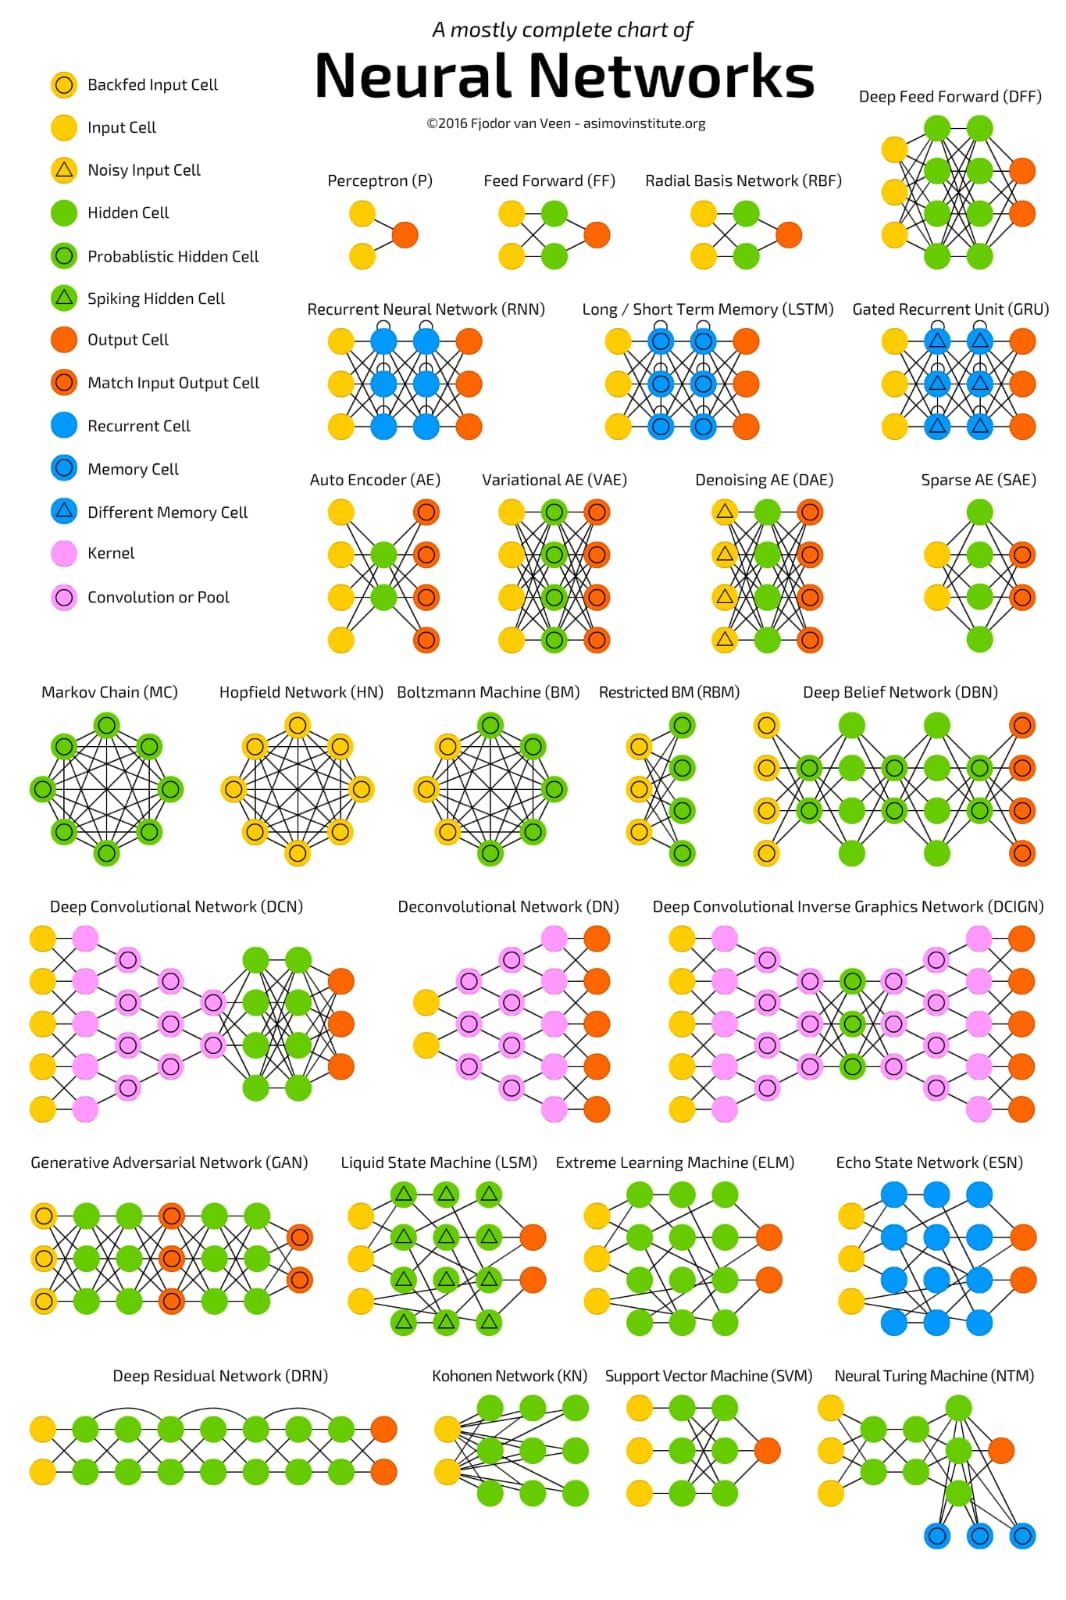
\includegraphics[width=0.9\textwidth]{imgs/neural_networks.jpeg}
  \caption{Panorama de arquiteturas de redes neurais \cite{asimov2017}}
  \label{fig:nnzoo}
\end{figure}

\FloatBarrier
\subsection{Large Language Models}

O funcionamento dos \textit{Large Language Models} (LLMs) envolve, inicialmente, uma fase de pré-treinamento sobre corpora textuais extensos e diversos. Nessa etapa, o modelo aprende representações estatísticas das palavras e suas relações contextuais. Subsequentemente, o modelo pode ser refinado por meio de técnicas de ajuste fino (\textit{fine-tuning}) para tarefas ou domínios específicos, como medicina, direito ou engenharia de software. Essa adaptação permite que o modelo adquira conhecimento especializado e aprimore seu desempenho em aplicações particulares \cite{jelodar2025, ouyang2023}.

Uma das características mais notáveis dos LLMs é sua capacidade de realizar generalização em tarefas para as quais não foram explicitamente programados. Isso ocorre porque, durante o treinamento, os modelos aprendem padrões sintáticos, semânticos e pragmáticos da linguagem, o que os capacita a inferir intenções, completar sentenças e até mesmo gerar respostas inéditas com base em instruções ambíguas ou vagas \cite{liu2024hallucinations, fan2023llmsw}.

Nesse sentido, no contexto da engenharia de software, os LLMs têm sido amplamente empregados para atividades como compreensão de requisitos, geração de código, documentação automatizada e verificação semântica. Tais aplicações se beneficiam da habilidade dos modelos em transitar entre linguagem natural e linguagem de programação, estabelecendo uma ponte entre a comunicação humana e a lógica computacional. Conforme apontado por \citeonline{jelodar2025}, o uso de LLMs em tarefas de análise de código tem-se mostrado promissor por sua capacidade de capturar estruturas semânticas profundas e apoiar a automação de tarefas críticas em ambientes de desenvolvimento.

Em suma, os LLMs representam um avanço significativo na interseção entre inteligência artificial e linguagem, oferecendo uma base tecnológica versátil para a construção de sistemas inteligentes capazes de compreender e manipular texto com sofisticação crescente.

\subsection{Arquitetura Transformer}

O avanço dos LLMs está intrinsecamente ligado à evolução de suas arquiteturas. Entre as diversas estruturas propostas, a arquitetura \textit{Transformer} representa um marco fundamental na história do processamento de linguagem natural, estabelecendo as bases dos modelos contemporâneos mais poderosos, como BERT, GPT e LaMDA.

A arquitetura Transformer foi projetada para resolver tarefas de transdução de sequência, como a tradução automática, de maneira mais eficiente que os modelos recorrentes anteriores, como RNNs e LSTMs. O elemento central do Transformer é o mecanismo de atenção, especialmente a \textit{self-attention}, que permite ao modelo capturar dependências contextuais entre quaisquer partes da entrada, independentemente de sua distância posicional, superando limitações comuns às redes recorrentes no aprendizado de relações de longo alcance no texto \cite{vaswani2017}.

A arquitetura original é composta por dois componentes principais: o codificador (\textit{encoder}) e o decodificador (\textit{decoder}). Ambos consistem em múltiplas camadas empilhadas, sendo que cada camada do codificador contém dois subcomponentes: um mecanismo de atenção multi-cabeça (\textit{multi-head attention}) e uma rede \textit{feedforward} totalmente conectada. O decodificador, por sua vez, incorpora um terceiro mecanismo de atenção, chamado \textit{encoder-decoder attention}, que permite integrar as representações aprendidas pelo codificador na geração das saídas \cite{ankit2024transformer}.  Essa estrutura pode ser visualizada na Figura~\ref{fig:transformer}, que ilustra a disposição dos principais componentes da arquitetura Transformer proposta por \citeonline{vaswani2017}

\begin{figure}[H]
    \centering
    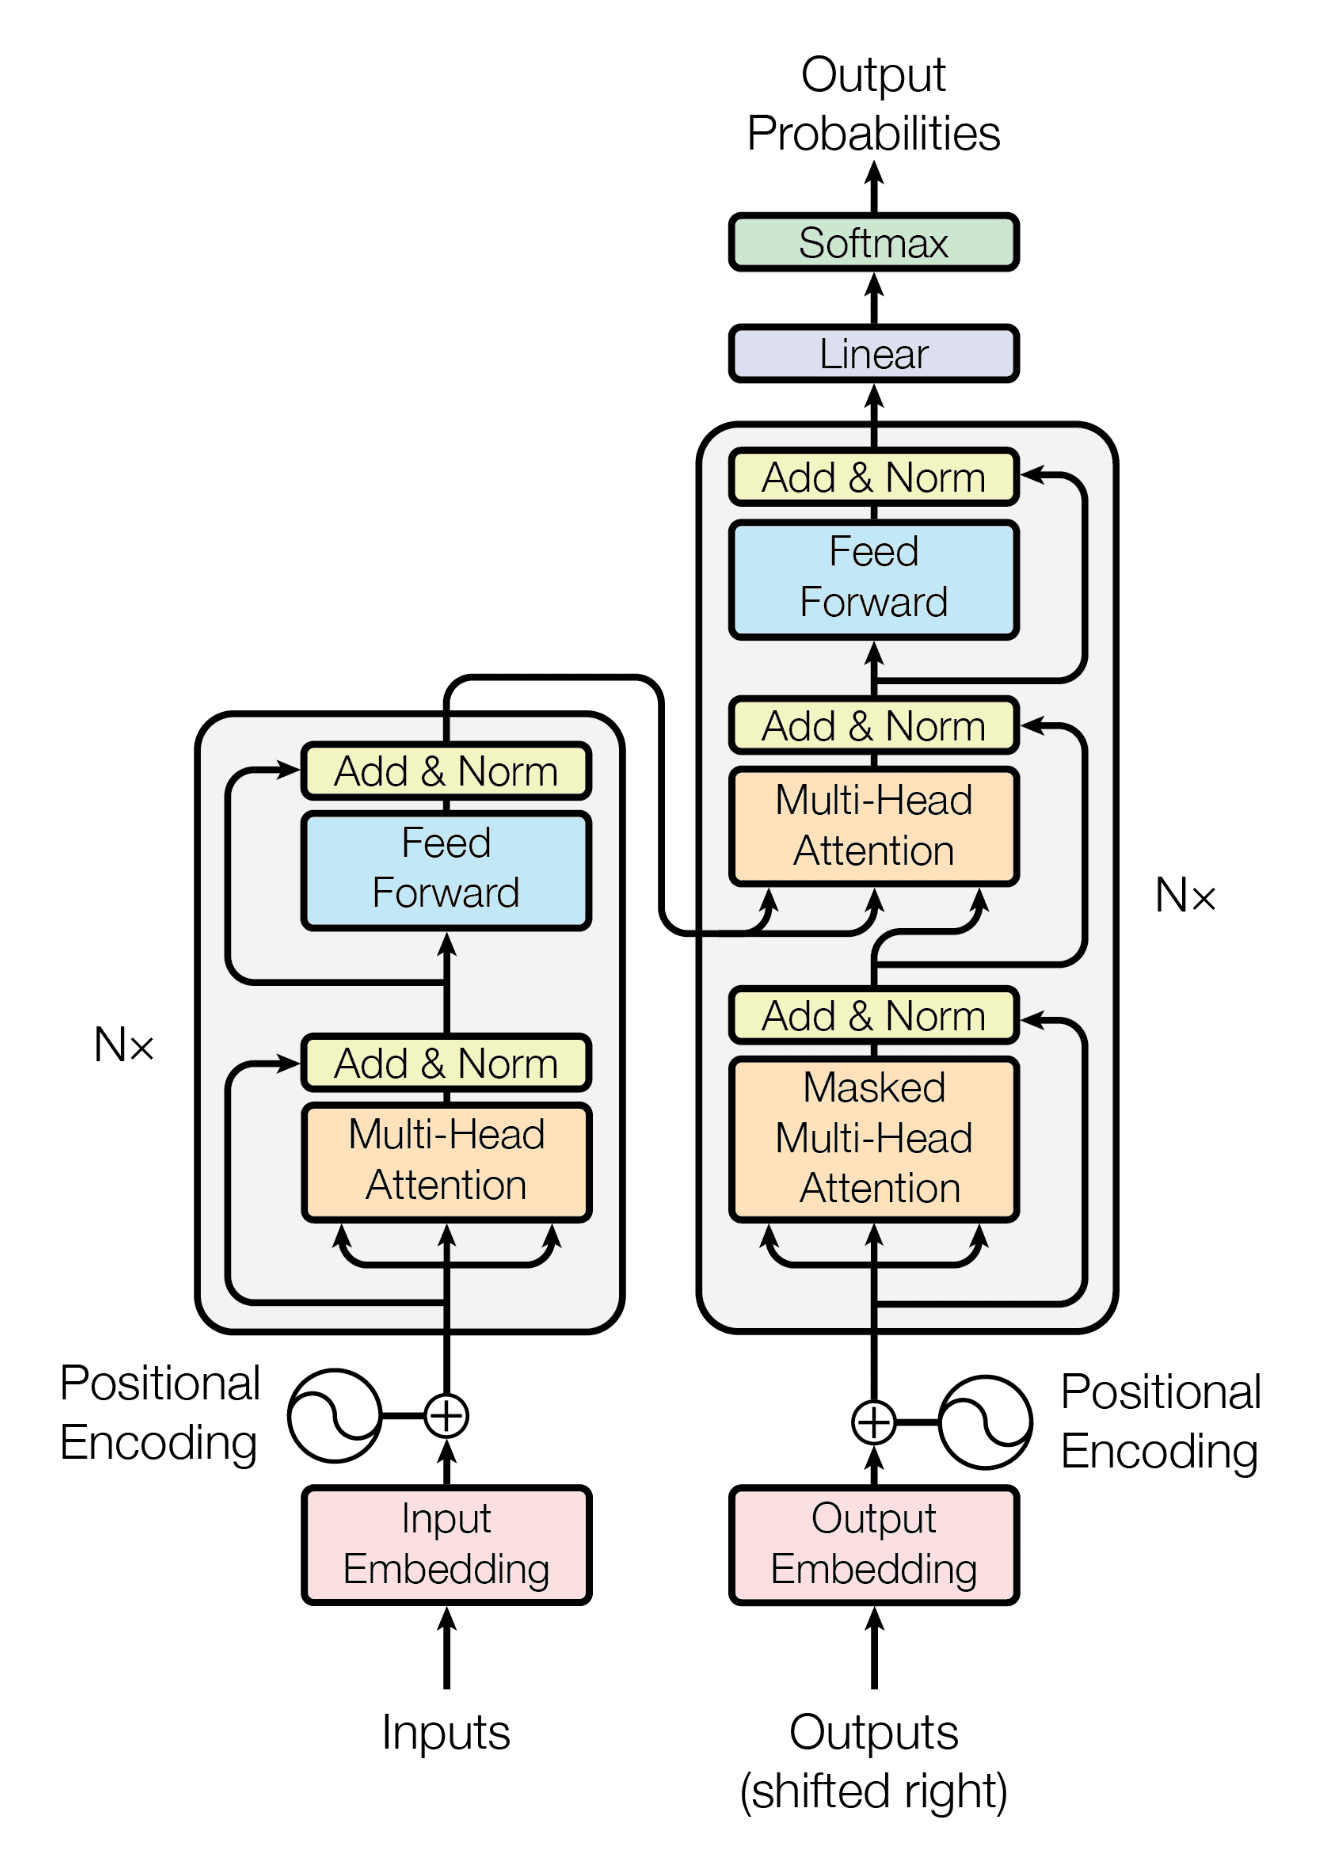
\includegraphics[width=0.75\textwidth]{imgs/transformer.png}
    \caption{Arquitetura do modelo Transformer \cite{vaswani2017}}
    \label{fig:transformer}
\end{figure}


Um dos aspectos mais inovadores do Transformer é a sua natureza altamente paralelizável, possibilitando ganhos significativos em desempenho computacional. Diferentemente das RNNs, que processam dados de forma sequencial, o Transformer permite o processamento simultâneo de todos os elementos da sequência de entrada, aproveitando de forma mais eficiente a arquitetura paralela das GPUs modernas \cite{ankit2024transformer}.

Para representar a ordem dos \textit{tokens} já que o modelo não possui uma estrutura sequencial intrínseca, são utilizados codificadores posicionais (\textit{positional encodings}), geralmente baseados em funções senoidais e cossenoidais de frequências variadas, os quais são somados aos vetores de \textit{embeddings} dos \textit{tokens} \citeonline{vaswani2017}. Essa codificação permite ao modelo inferir relações posicionais relativas entre os elementos da sequência.

Cada mecanismo de atenção da arquitetura é implementado por meio da chamada \textit{Scaled Dot-Product Attention}, onde o vetor de consulta (\textit{query}) é comparado com os vetores de chave (\textit{key}), e os resultados ponderam os vetores de valor (\textit{value}) para determinar a relevância contextual de cada \textit{token}. Esse processo é repetido em múltiplas cabeças de atenção (\textit{multi-head}), permitindo que o modelo aprenda diferentes aspectos das relações semânticas em paralelo \cite{ankit2024transformer, raschka2025bigllm}.

A partir da arquitetura original, diversas variantes e otimizações foram propostas. Modelos como GPT, BERT e T5 introduziram variações no uso do codificador, decodificador ou ambos, bem como aprimoramentos em camadas de normalização, mecanismos de atenção e escalabilidade. Além disso, técnicas como o uso de \textit{Mixture-of-Experts} (MoE), \textit{Grouped Query Attention} (GQA) e mecanismos de janela deslizante (\textit{sliding window attention}) foram desenvolvidas para aumentar a capacidade dos modelos e, ao mesmo tempo, reduzir os custos computacionais durante a inferência \citeonline{raschka2025bigllm}.

Esses avanços demonstram que, embora a estrutura base do Transformer permaneça amplamente utilizada, sua flexibilidade arquitetônica possibilitou diversas inovações. Atualmente, a arquitetura Transformer constitui a espinha dorsal da maioria dos LLMs de alto desempenho, permitindo não apenas avanços em tarefas linguísticas, mas também sua aplicação em domínios multimodais, como imagens, vídeos e interações conversacionais \cite{ankit2024transformer, raschka2025bigllm}.


\subsection{Janela de Contexto}

A janela de contexto de um modelo de linguagem representa a quantidade de informações textuais que o modelo é capaz de processar simultaneamente. Trata-se de um parâmetro crucial para tarefas que envolvem raciocínio sobre longos documentos, como verificação de requisitos em código-fonte, sumarização e busca semântica. O tamanho e o funcionamento da janela de contexto têm implicações diretas na eficácia e nas limitações dos modelos de linguagem natural, particularmente os baseados na arquitetura Transformer.

O modelo Transformer, proposto por \citeonline{vaswani2017}, introduziu o mecanismo de autoatenção como forma de modelar dependências globais entre \textit{tokens} sem recorrer a estruturas sequenciais como RNNs. Cada \textit{token} pode se conectar com qualquer outro \textit{token} da sequência por meio de uma matriz de atenção, o que implica em uma complexidade quadrática em relação ao tamanho da entrada. Embora isso permita modelar dependências de longo alcance com eficiência teórica, o custo computacional impõe limites práticos ao comprimento da janela de contexto suportada.

Para contornar essa limitação, estratégias como o \textit{chunking} (divisão de textos em segmentos menores) passaram a ser adotadas em sistemas de Recuperação Aumentada por Geração (RAG). Contudo, o \textit{chunking} tradicional, no qual os trechos são vetorizados separadamente, pode causar a perda de contexto semântico. Para enfrentar esse desafio, \citeonline{gunther2025} propuseram o método \textit{Late Chunking}, que primeiro vetoriza todo o documento com modelos de contexto longo e, só depois, aplica o agrupamento para o cálculo das representações vetoriais dos \textit{chunks}. Isso permite que os vetores reflitam a semântica global do documento, superando a limitação contextual dos métodos tradicionais.

Além disso, \citeonline{jin2024} propuseram o método \textit{SelfExtend}, que demonstra que modelos com codificações posicionais relativas, como RoPE, possuem capacidades inatas para processar sequências mais longas do que aquelas observadas durante o treinamento. A técnica consiste em modificar a atenção de forma que posições relativas fora da distribuição original sejam mapeadas para valores já observados, estendendo efetivamente a janela de contexto sem necessidade de \textit{fine-tuning}. Isto é especialmente relevante para tarefas que requerem consistência contextual em documentos extensos, como a análise de requisitos de software dispersos em arquivos distintos.

Ambas as abordagens mostram que a eficácia do modelo diante de textos longos depende não apenas do tamanho da janela de contexto, mas também da forma como a informação contextual é preservada e utilizada na geração dos \textit{embeddings}. Neste sentido, métodos como \textit{Late Chunking} e \textit{SelfExtend} tornam-se particularmente promissores para aplicações em que a rastreabilidade e a fidelidade semântica ao longo do texto são essenciais.

Por fim, destaca-se que o aproveitamento eficiente da janela de contexto é diretamente influenciado pelo design da arquitetura, pelas estratégias de vetorização e pela engenharia de \textit{prompts}. Assim, o estudo da janela de contexto é um componente fundamental para compreender os limites e as possibilidades dos modelos de linguagem em tarefas que envolvem grandes volumes de informação textual.

\subsection{Funcionamento e Parâmetros dos Modelos de Linguagem}

Os LLMs funcionam por meio de um processo dividido em duas fases: treinamento e geração. Na fase de treinamento, o modelo é exposto a grandes volumes de dados textuais e ajusta internamente seus parâmetros para aprender padrões linguísticos, sintáticos e semânticos. O número de parâmetros varia conforme o modelo, podendo atingir centenas de bilhões ou até trilhões, como é o caso do GPT-4, que apresenta arquitetura do tipo \textit{mixture-of-experts} com cerca de 1,8 trilhão de parâmetros \citeonline{openai2023}. Esses parâmetros são responsáveis por representar o conhecimento aprendido e são fixados após o treinamento. Na fase de inferência, por sua vez, o comportamento do modelo passa a ser governado por hiperparâmetros que controlam como as respostas são geradas a partir desse conhecimento prévio.

Entre esses hiperparâmetros, destaca-se a \textit{temperature}, que regula o grau de aleatoriedade da geração textual. Em termos práticos, valores baixos de \textit{temperature} (próximos de 0) resultam em respostas mais determinísticas, favorecendo a exatidão e a repetição de padrões aprendidos; por outro lado, valores mais altos (acima de 1.0) promovem maior diversidade e imprevisibilidade na escolha dos \textit{tokens} subsequentes. A configuração apropriada desse parâmetro é especialmente relevante em contextos técnicos, como a análise de requisitos de software, nos quais a fidelidade semântica e a consistência textual são essenciais \citeonline{renze2024}.

Outros parâmetros amplamente utilizados incluem o \textit{top-k} e o \textit{top-p}. O \textit{top-k} restringe a escolha do próximo \textit{token} aos `k` \textit{tokens} mais prováveis, limitando o espaço de amostragem e eliminando opções de baixa probabilidade, o que favorece a coesão em tarefas com vocabulário mais técnico ou padronizado \citeonline{holtzman2020}. O \textit{top-p}, também conhecido como \textit{nucleus sampling}, adota uma abordagem dinâmica ao selecionar o menor conjunto de \textit{tokens} cuja soma de probabilidades atinja um limite cumulativo (geralmente entre 0,8 e 0,95), permitindo um equilíbrio entre variedade e controle estatístico da geração \citeonline{fan2018}.

Além disso, penalidades de frequência e de presença são utilizadas para mitigar repetições, incentivando o uso de vocabulário mais diverso em textos extensos. Estas penalidades reduzem a probabilidade de reaparecimento de \textit{tokens} já utilizados, sendo particularmente úteis em aplicações que envolvem geração de documentação técnica, explicações ou justificativas complexas \citeonline{openai2023}.

A interação entre esses hiperparâmetros permite a adaptação do comportamento do modelo às necessidades específicas de diferentes tarefas. Por exemplo, na verificação automatizada de requisitos, recomenda-se utilizar \textit{temperature} baixa e \textit{top-p} moderado, a fim de priorizar a exatidão e reduzir alucinações. Já em tarefas de geração descritiva ou criativa, como a escrita de histórias de usuários ou a geração de testes automatizados com descrições narrativas, configurações mais permissivas favorecem a variabilidade sem comprometer a utilidade \citeonline{raffel2020}.

Embora tradicionalmente se associe a \textit{temperature} ao controle da “criatividade” de um modelo, estudos recentes indicam que sua influência é limitada em comparação com outros fatores, como a estrutura da tarefa ou o tipo de \textit{fine-tuning} aplicado \citeonline{nguyen2025}. Isso reforça a necessidade de compreender esses parâmetros como elementos que interagem entre si, exigindo ajustes experimentais cuidadosos conforme o domínio de aplicação.

Dessa forma, os parâmetros de decodificação exercem papel central na fase de inferência dos modelos de linguagem, moldando o estilo, a coerência e a adequação da saída gerada. No contexto de engenharia de software, em especial na análise de conformidade de requisitos, sua correta configuração é essencial para garantir não apenas a relevância da resposta, mas também a rastreabilidade semântica e a consistência técnica com os artefatos analisados.

\subsection{Embedding, Chunk e Vetorização}

O uso de \textit{embeddings} vetoriais tem se consolidado como uma abordagem essencial no processamento de linguagem natural (PLN), especialmente no contexto de LLMs. A técnica consiste na transformação de dados textuais não estruturados em vetores de alta dimensionalidade que capturam semântica e contexto, permitindo que sistemas computacionais realizem tarefas como busca semântica, recuperação de informações e verificação de similaridade com maior eficiência \citeonline{lema2025}.

O processo de vetorização normalmente se inicia com a fragmentação do conteúdo textual em segmentos menores, denominados \textit{chunks}. Esses \textit{chunks} são projetados para respeitar os limites da janela de contexto do modelo, otimizando a capacidade de raciocínio e minimizando a perda de informação semântica. A definição do tamanho do \textit{chunk} deve equilibrar a granularidade da análise e a eficiência da indexação, sendo comum a adoção de janelas de 512 a 1024 \textit{tokens} em aplicações práticas \citeonline{muennighoff2022}.

Uma vez definidos, os \textit{chunks} são processados por modelos de \textit{embedding}, os quais produzem representações vetoriais que preservam relações semânticas e sintáticas entre os textos originais. No caso do SGPT, por exemplo, é aplicada uma técnica de \textit{weighted mean pooling} sobre os estados ocultos dos \textit{tokens}, ponderando a influência de \textit{tokens} mais à frente na sequência, uma vez que o modelo é baseado em atenção causal \citeonline{muennighoff2022}. Esta abordagem demonstrou superioridade em tarefas de busca semântica simétrica e assimétrica, com ganhos de desempenho notáveis quando comparados a \textit{embeddings} tradicionais.

Após a geração dos \textit{embeddings}, esses vetores são armazenados em bases de dados vetoriais (\textit{Vector Databases} – VDBs), que viabilizam operações de similaridade por meio de técnicas de busca aproximada ao vizinho mais próximo (\textit{Approximate Nearest Neighbor Search} – ANNS). Tais técnicas utilizam estruturas como índices hierárquicos, árvores k-d, grafos navegáveis e particionamentos baseados em quantização para permitir a recuperação eficiente mesmo em cenários de altíssima dimensionalidade \citeonline{lema2025}. Essa arquitetura é particularmente relevante para aplicações que requerem resposta em tempo real ou processamento em larga escala, como nos sistemas de Recuperação Aumentada por Geração (RAG) empregados em soluções corporativas e agentes autônomos.

A eficácia do processo de vetorização não depende apenas do modelo utilizado para gerar os \textit{embeddings}, mas também de boas práticas no pré-processamento textual, como a remoção de ruídos e a padronização da linguagem. Além disso, a forma como os \textit{chunks} são segmentados influencia diretamente na manutenção do contexto e da coerência semântica ao longo dos vetores gerados \citeonline{muennighoff2022}. Outro aspecto importante é a aplicação de técnicas de normalização nos vetores, como a normalização L2, que garante que as métricas de similaridade permaneçam matematicamente consistentes e comparáveis em grandes volumes de dados \citeonline{lema2025}.

A integração dessas tecnologias tem permitido o desenvolvimento de sistemas inteligentes capazes de realizar busca semântica de alta precisão, detecção de duplicidade textual, verificação de conformidade entre requisitos e código-fonte, bem como sumarização e rastreabilidade de informações em \textit{pipelines} automatizados de engenharia de software.

\subsection{Engenharia de Prompt e Protocolo MCP}

A engenharia de \textit{prompt} tem emergido como uma prática central na interação com LLMs, sendo especialmente relevante em contextos empresariais e acadêmicos. Essa técnica consiste na formulação de instruções textuais com o objetivo de elicitar comportamentos específicos dos modelos, como sumarização, classificação, geração de código e análise de documentos. \citeonline{desmond2024} destacam que, embora o uso de linguagem natural sugira uma interação intuitiva, a construção de \textit{prompts} eficazes exige conhecimento técnico, compreensão do funcionamento interno dos modelos e uma abordagem iterativa.

Estudos conduzidos por \citeonline{kin2023} apontam que usuários frequentemente cometem erros conceituais ao tentar interagir com LLMs, o que evidencia a necessidade de ferramentas e metodologias que auxiliem na criação de \textit{prompts} mais robustos. Complementarmente, \citeonline{braun2024} propõem uma taxonomia dos componentes do \textit{prompt}, destacando a importância do refinamento das instruções e da adaptação do conteúdo contextual.

Pesquisas empíricas demonstram que usuários experientes costumam ajustar elementos do \textit{prompt} como a instrução da tarefa, o contexto fornecido e o formato esperado da resposta. De acordo com \citeonline{desmond2024}, as alterações mais frequentes incluem modificações semânticas, adição de exemplos e reestruturações de formato. Além disso, estratégias avançadas têm se mostrado eficazes em tarefas complexas, como o \textit{few-shot prompting}, que consiste em fornecer alguns exemplos da tarefa desejada para guiar o modelo, e o \textit{chain-of-thought}. Esta última técnica é definida pelo "encadeamento de raciocínio" no \textit{prompt}, o que, segundo \citeonline{wei2022}, auxilia na execução de tarefas que requerem múltiplas etapas cognitivas. Em outra abordagem, \citeonline{melamed2023} tratam o design de \textit{prompts} como um problema inverso, propondo modelos que otimizam automaticamente sua estrutura para maximizar a performance.

A complexidade da engenharia de \textit{prompt} aumenta quando se busca garantir rastreabilidade entre os requisitos expressos em linguagem natural e os artefatos de software correspondentes. Nesse contexto, destaca-se o uso do \textit{Model Context Protocol} (MCP) como um mecanismo padronizado que organiza a comunicação entre modelos de linguagem e sistemas externos. O MCP opera em uma arquitetura cliente-servidor, onde aplicações de IA (\textit{hosts}) se conectam a servidores MCP especializados para obter dados contextuais relevantes. Esses servidores podem disponibilizar ferramentas, recursos e \textit{prompts} estruturados, que são acessados dinamicamente pelos modelos durante a execução de tarefas.

O protocolo é dividido em duas camadas principais: a camada de dados, baseada em JSON-RPC 2.0, que define como tarefas, respostas e recursos são trocados; e a camada de transporte, responsável pela conexão e autenticação, que pode funcionar via STDIO para servidores locais ou HTTP para servidores remotos \citeonline{mcp2024}.

Ao integrar a engenharia de \textit{prompt} com o MCP, é possível criar fluxos interativos e auditáveis nos quais os modelos obtêm contexto em tempo real, executam ferramentas externas ou acessam bases de conhecimento estruturadas com alta rastreabilidade. Essa abordagem fortalece a confiabilidade das LLMs em tarefas críticas, como análise de requisitos de software, verificação de conformidade e geração automatizada de artefatos técnicos.


\subsection{Agentes de Inteligência Artificial}


Agentes de Inteligência Artificial (IA) são entidades autônomas de software projetadas para executar tarefas específicas de forma adaptativa, racional e contínua. Fundamentados em ciclos de percepção, raciocínio e ação, esses agentes analisam entradas do ambiente (digitais ou físicos), tomam decisões com base em regras, heurísticas ou modelos treinados, e atuam para atingir metas estabelecidas. Diferentemente de assistentes baseados apenas em prompts ou scripts determinísticos, os agentes de IA modernos possuem certo grau de autonomia operacional, podendo interagir com APIs, sistemas de arquivos, modelos de linguagem e bancos de dados (IBM, 2024; AWS, 2024).

Com o avanço dos modelos fundacionais, especialmente os LLMs, esses agentes passaram a incorporar mecanismos de raciocínio natural, recuperação semântica e execução contextualizada de comandos. Isso os torna aptos a realizar tarefas como responder perguntas, sintetizar documentos, realizar buscas, chamar funções externas, interpretar imagens, gerar relatórios ou interagir com sistemas complexos de forma autônoma (Sapkota et al., 2025). Aplicações práticas incluem assistentes corporativos inteligentes, bots de atendimento, análise automatizada de requisitos de software e agentes robóticos embarcados. Empresas como AWS, Google, IBM e Microsoft já adotam arquiteturas baseadas em agentes para orquestração de tarefas entre serviços internos e externos.

A IBM (2024) propõe uma arquitetura modular baseada em três elementos principais: um plano de raciocínio e tomada de decisão; um componente de memória para estado e contexto; e um executor que interage com ferramentas, sistemas e APIs. Essa estrutura permite que o agente seja continuamente invocado por eventos, mantenha persistência sobre tarefas anteriores e adapte seu comportamento a partir do histórico. Além disso, agentes podem ser organizados em sistemas cooperativos, uma abordagem conhecida como Agentic AI  em que múltiplos agentes especializados trabalham de forma coordenada para resolver problemas complexos, com divisão de tarefas, comunicação entre agentes e reuso de memória compartilhada (Sapkota et al., 2025).

O conceito de Agentic AI amplia a atuação dos agentes convencionais ao introduzir estruturas colaborativas compostas por unidades autônomas com papéis distintos. Tais agentes são capazes de operar em camadas distintas, como planejadores, executores ou verificadores, interagindo entre si para atingir metas coletivas de forma eficaz. Ferramentas como AutoGen, CrewAI e LangGraph já exploram esse paradigma, permitindo a criação de pipelines autônomos, fluxos de raciocínio distribuído e agentes capazes de coordenar ações em ambientes híbridos físicos-digitais com alto grau de adaptabilidade (Sapkota et al., 2025).

\xchapter{Desenvolvimento}{}

\section{Abordagem Geral}
Este trabalho adota uma abordagem de natureza aplicada e qualitativa, fundamentada em um experimento controlado com artefatos de um software real. O objetivo central consiste em investigar a eficácia de Modelos de Linguagem de Larga Escala  na verificação automatizada da conformidade entre requisitos, expressos em linguagem natural, e sua respectiva implementação no código-fonte. A metodologia proposta segue um fluxo estruturado que compreende a extração de arquivos de um repositório Git, a construção e o refinamento de prompts e, por conseguinte, a aplicação destes a diferentes modelos de linguagem por meio da ferramenta Gemini CLI e do GitHub Copilot integrado ao Visual Studio Code. As atividades foram conduzidas em um projeto concreto — o sistema “Nivelamento Online”, desenvolvido pela empresa Exatamente Soluções Educacionais, o que confere realismo e aplicabilidade prática à análise. Nesse contexto, busca-se avaliar a precisão das inferências geradas pelos modelos, os efeitos da engenharia de prompt e o impacto de distintas arquiteturas e configurações sobre a qualidade da verificação.

\section{Caracterização do Sistema sob Estudo}

O \textit{Nivelamento Online} (NiO) é uma plataforma educacional gamificada desenvolvida para apoiar o reforço de conteúdos escolares por meio de quizzes e atividades interativas. O sistema oferece modos de uso individual e coletivo, com funcionalidades voltadas tanto ao aluno quanto ao professor, incluindo a criação de perguntas, acompanhamento de desempenho e recursos de motivação baseados em mecânicas de jogo. 

Sua implementação adota a estrutura de múltiplos projetos, sendo os módulos de front-end e back-end os princiapis, além desses o repositório inclui outros componentes auxiliares relacionados à operação da plataforma. O front-end é construído como uma aplicação de página única (SPA) utilizando o framework Vue.js, sendo responsável pela interface e experiência do usuário. O back-end principal, por sua vez, é desenvolvido em Java com Spring Boot sendo dividido em multi módulos. Essa estrutura modular e multifacetada confere ao sistema uma complexidade significativa, especialmente no que diz respeito à rastreabilidade entre requisitos e implementações.

\section{Metodologia}

O percurso metodológico deste trabalho foi fundamentado em um processo iterativo, estruturado em seis etapas principais. Cada etapa representa uma fase distinta do experimento de verificação automatizada da conformidade entre requisitos e código-fonte, conforme descrito a seguir. 

\begin{enumerate}
    \item \textbf{Coleta de Artefatos:} A fase inicial consistiu na extração dos artefatos do sistema “Nivelamento Online”, diretamente de seu repositório Git. Foram coletados tanto os documentos de requisitos quanto os arquivos de código-fonte que serviram de base para o experimento. 
    \item \textbf{Formulação Inicial dos Prompts:} Com base nos requisitos, elaboraram-se prompts iniciais em linguagem natural, cujo propósito era instruir os modelos de linguagem a verificar a implementação de cada requisito. Tais prompts foram projetados para que os modelos classificassem os requisitos em categorias predefinidas (\textit{Implemented}, \textit{Partially}, \textit{Missing} ou \textit{Unknown}) e justificassem suas conclusões. 
    \item \textbf{Execução Inicial com LLMs:} Subsequentemente, os prompts foram submetidos a diferentes modelos de linguagem por meio da ferramenta Gemini CLI e, paralelamente, via GitHub Copilot no Visual Studio Code. Essa execução inicial estabeleceu uma linha de base para a avaliação de desempenho. 
    \item \textbf{Refinamento com Engenharia de Prompt:} A análise dos resultados preliminares permitiu identificar falhas interpretativas e limitações. Diante disso, os prompts foram aprimorados com o uso de técnicas de engenharia de prompt, como \textit{few-shot prompting} (inserção de exemplos) e \textit{chain-of-thought prompting} (estímulo ao raciocínio em cadeia), objetivando maior robustez e rastreabilidade semântica. 
    \item \textbf{Reexecução com Prompts Refinados:} Os prompts otimizados foram então reaplicados aos mesmos modelos e ambientes. Essa etapa foi crucial para comparar diretamente o desempenho antes e depois do refinamento, permitindo, assim, mensurar o impacto das técnicas de engenharia de prompt. 
    \item \textbf{Coleta e Análise dos Resultados:} Por fim, todas as respostas geradas foram sistematicamente registradas, categorizadas e avaliadas. As análises abrangeram a validação das respostas e a medição da acurácia, taxa de omissão, precisão, \textit{recall} e \textit{F1-score}. Essas métricas foram utilizadas por serem amplamente reconhecidas na literatura como indicadores robustos para avaliar classificadores, permitindo mensurar não apenas a proporção de acertos, mas também a capacidade dos modelos em evitar falsas classificações e identificar corretamente os requisitos relevantes. Os dados foram consolidados em tabelas de desempenho para viabilizar uma interpretação quantitativa e qualitativa do comportamento dos modelos.
\end{enumerate}

% A utilização de métricas quantitativas revelou-se essencial para avaliar objetivamente o desempenho dos modelos aplicados à verificação automatizada de conformidade entre requisitos e código-fonte. Neste experimento, duas métricas foram particularmente relevantes: a acurácia e a taxa de omissão. A acurácia permite mensurar a proporção de classificações corretas, isto é, em que o modelo atribuiu o rótulo adequado ao requisito analisado, em relação ao total de casos avaliados. Trata-se de uma métrica abrangente, que fornece uma visão geral da performance do modelo, considerando tanto acertos em requisitos implementados quanto corretamente identificados como ausentes. 

% Já a taxa de omissão foi empregada para capturar um tipo específico de falha: situações em que o modelo não forneceu nenhuma resposta em requisitos cuja implementação estava de fato presente no código. Em contextos de engenharia de software, esse tipo de erro pode comprometer significativamente a rastreabilidade e a confiabilidade do processo de auditoria, ao deixar requisitos efetivamente atendidos sem o devido reconhecimento. Assim, a análise combinada da acurácia e da taxa de omissão fornece uma visão crítica sobre a capacidade do modelo de não apenas acertar, mas também de evitar silêncios injustificados diante de evidências válidas.

\subsection{Seleção dos casos de teste.}
Para condução do experimento, foram selecionados dois documentos de caso de teste provenientes de módulos distintos do sistema. O primeiro corresponde à funcionalidade de geração automatizada de questões com apoio de Inteligência Artificial, a qual envolve tanto componentes de \textit{back-end} quanto de \textit{front-end}, sendo referenciada nos testes como módulo \textbf{IA}. Essa funcionalidade permite que o usuário submeta um documento contendo conteúdo pedagógico ou uma descrição textual, com o objetivo de que a IA extraia automaticamente questões coerentes com o material fornecido e as insira diretamente na base de dados do sistema. Trata-se, portanto, de uma funcionalidade que combina processamento textual, análise semântica e integração com o fluxo de criação de atividades dentro da plataforma.

O segundo módulo selecionado, identificado como \textbf{REL}, refere-se à geração de relatórios de desempenho de alunos ou jogadores. Embora o sistema já ofereça visualizações gráficas e estatísticas no ambiente online, essa funcionalidade foi desenvolvida para permitir que professores ou organizadores exportem os dados consolidados em um arquivo no formato \texttt{.xlsx}, compatível com softwares de planilha. Essa opção proporciona uma visão abrangente, offline e reutilizável dos dados, o que é especialmente útil para análise detalhada, arquivamento ou compartilhamento externo dos resultados. A implementação do módulo REL encontra-se majoritariamente no \textit{back-end}, concentrando-se em operações de consulta, agregação e formatação dos dados educacionais.

Esses dois módulos foram escolhidos por representarem tipos distintos de desafio técnico, um com foco em integração com IA e requisição assíncrona, e outro com lógica de negócio intensiva no servidor e alto valor analítico. Os documentos de teste correspondentes serviram como base para a extração dos requisitos e cenários avaliados pelas IAs, e seus identificadores foram mantidos nos resultados (\texttt{IA-RF01}, \texttt{REL-RF02}, etc.) para permitir o rastreio da origem durante a análise.

\section{Visão Arquitetural da Solução}

Para contextualizar a solução proposta, foi utilizado o modelo C4, que permite representar a arquitetura de software em diferentes níveis de abstração. As Figuras~\ref{fig:c4_contexto} e~\ref{fig:c4_containers} apresentam, respectivamente, os diagramas de contexto e de containers, que, juntos, oferecem uma visão geral do fluxo operacional da solução e da organização de seus principais componentes.

\begin{figure}[H]
    \centering
    \begin{adjustbox}{width=0.9\textwidth,center}
        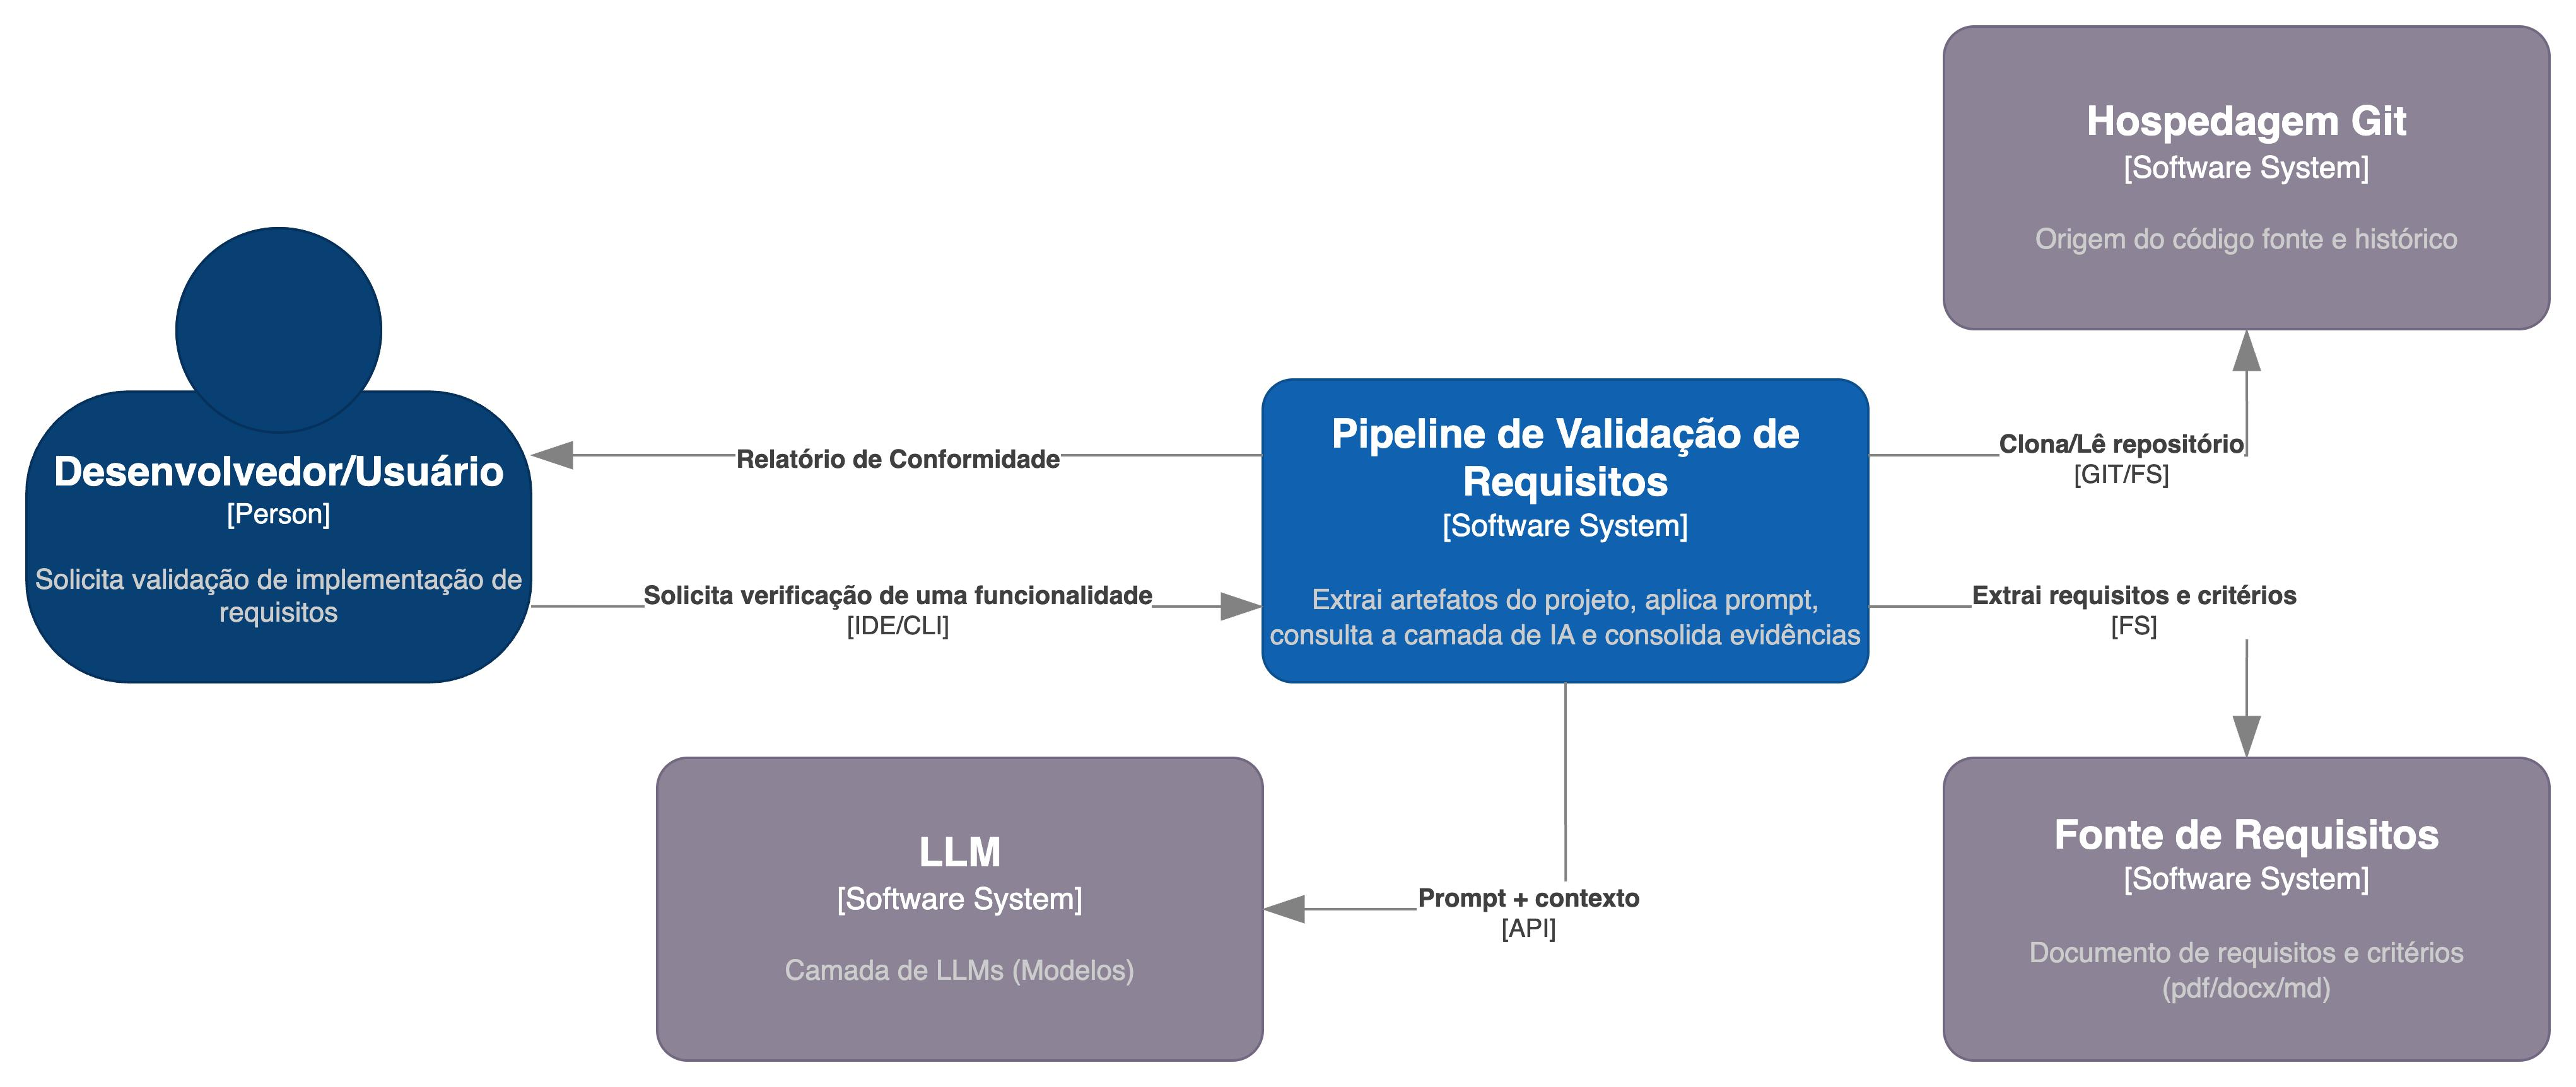
\includegraphics{imgs/c4_context.jpeg}
    \end{adjustbox}
    \caption{Diagrama de Contexto (Fonte: Própria)}
    \label{fig:c4_contexto}
\end{figure}

\begin{figure}[H]
    \centering
    \begin{adjustbox}{width=1.0\textwidth,center}
        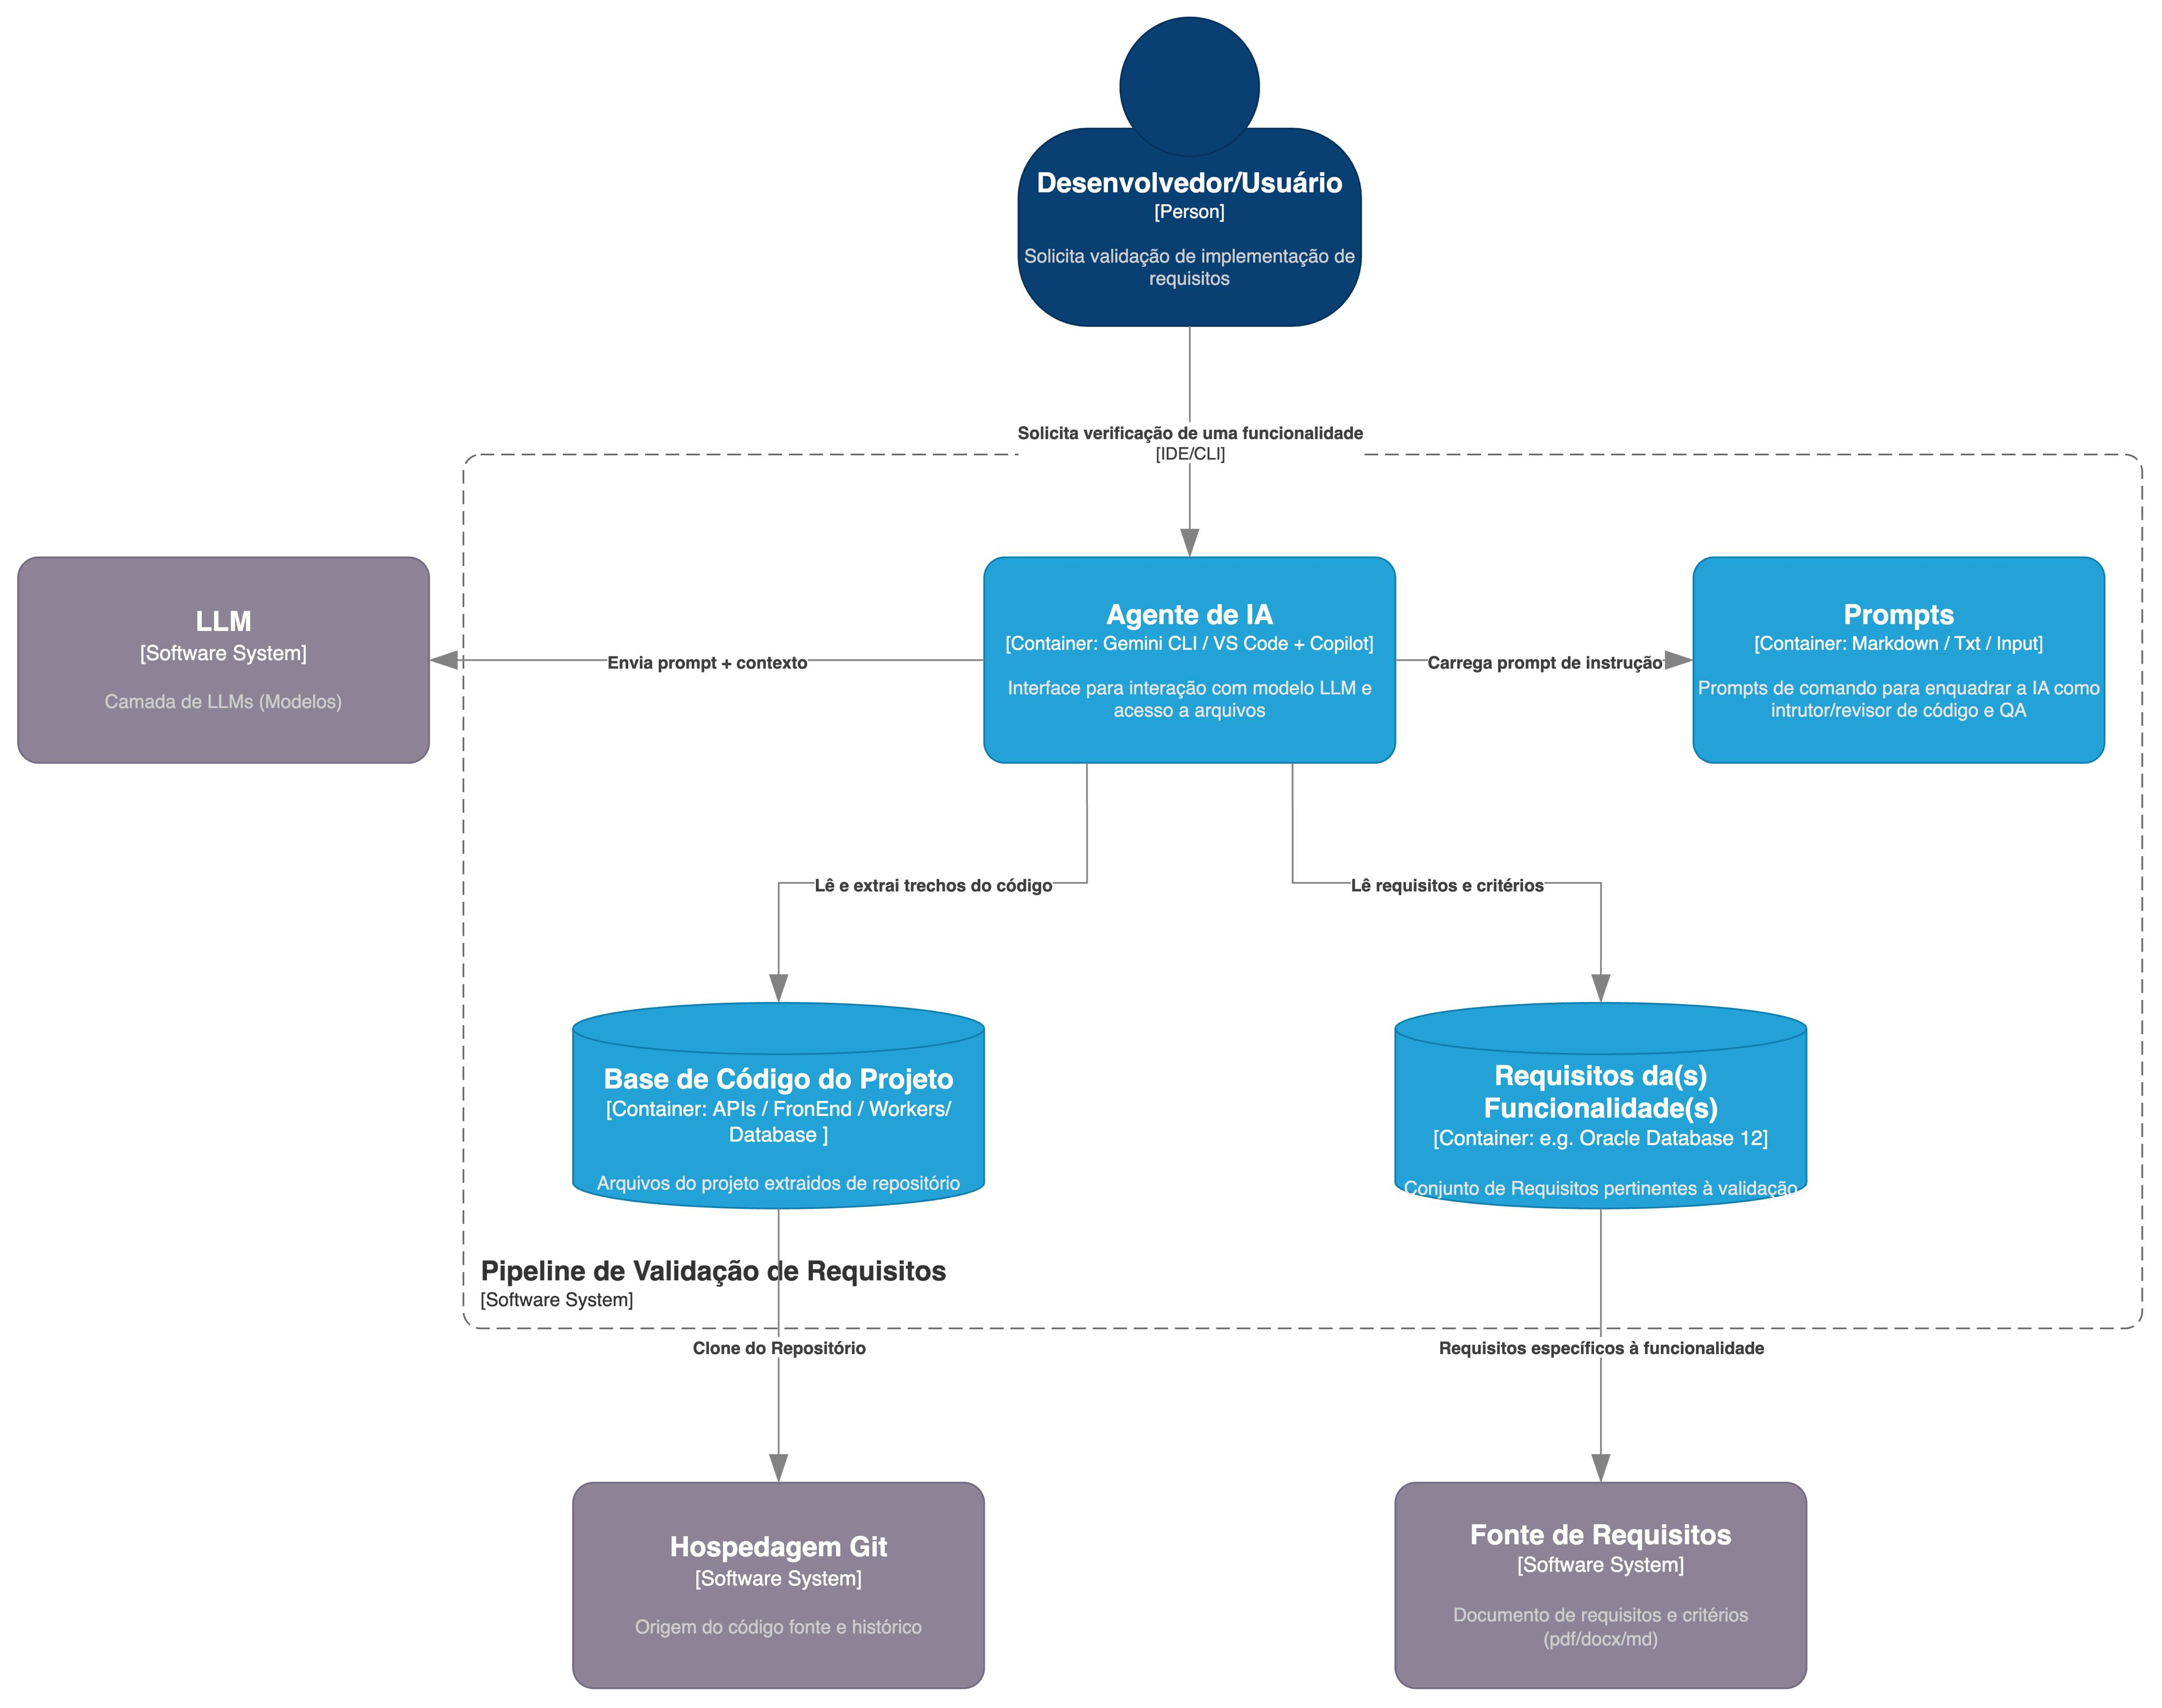
\includegraphics{imgs/c4_container.jpeg}
    \end{adjustbox}
    \caption{Diagrama de Containers (Fonte: Própria)}
    \label{fig:c4_containers}
\end{figure}

No diagrama de contexto (Figura~\ref{fig:c4_contexto}), observa-se que o processo tem início com a ação do usuário, que deseja validar se uma determinada funcionalidade foi implementada de acordo com os requisitos estabelecidos. Para isso, o usuário interage diretamente com o projeto local por meio de uma interface de linha de comando (CLI) ou uma interface gráfica no Ambiente de Desenvolvimento Integrado (IDE), ativando um conjunto estruturado de ações aqui denominado pipeline de validação de requisitos.

Essa pipeline consiste em operações realizadas localmente, como a leitura de arquivos do código-fonte e dos documentos de requisitos combinadas à construção de prompts, os quais serão utilizados como entrada para um modelo de linguagem (LLM), acessado remotamente via API. O modelo, por sua vez, retorna julgamentos ou explicações a respeito da conformidade entre os requisitos e os trechos de código analisados.

A Figura~\ref{fig:c4_containers} complementa essa visão ao detalhar os principais containers que participam do processo. O Agente de IA é representado como a interface de operação (CLI ou IDE), responsável por orquestrar o fluxo de validação, acessando diretamente os prompts, a base de código do projeto e os requisitos extraídos. Esse agente é responsável por preparar e enviar os dados ao modelo de linguagem, bem como interpretar as respostas e auxiliar na construção do relatório.

A base de código e os requisitos utilizados no processo são oriundos de repositórios hospedados externamente e previamente clonados ou armazenados na máquina local do usuário. Os prompts, por sua vez, são arquivos configuráveis (em Markdown ou texto estruturado) que orientam a atuação do agente como revisor, auditor ou verificador de conformidade.

Dessa forma, os dois diagramas apresentados fornecem uma visão consolidada do funcionamento da solução: um processo interativo, acionado localmente pelo usuário, que utiliza modelos de linguagem para auxiliar na análise semântica da aderência entre os requisitos documentados e o código-fonte implementado.


\subsection{Ferramentas e Modelos Utilizados}

O ambiente experimental foi configurado para permitir a comparação de desempenho entre diferentes modelos de linguagem de ponta, acessados por meio de duas interfaces principais. A seleção de múltiplos modelos visa observar variações na capacidade de interpretação e análise de código, conforme delineado nos objetivos específicos deste trabalho.

As ferramentas e os respectivos modelos utilizados foram:

\begin{itemize}
    \item Gemini CLI: Interface de linha de comando utilizada para interagir diretamente com o modelo Gemini 2.5 Pro.
    \item GitHub Copilot (integrado ao Visual Studio Code): A extensão foi configurada para alternar entre os seguintes modelos de apoio: Gemini 2.5 Pro, Claude Sonnet 4 e GPT 5.
\end{itemize}

Todos os testes foram executados mantendo os hiperparâmetros e configurações padrão dos modelos, a fim de garantir uma base de comparação consistente.


\section{Estruturação da Solução e Etapas do Experimento}
O sistema sob avaliação organiza, em um mesmo repositório, os módulos de \textit{front-end}, múltiplos serviços de \textit{back-end} e componentes adicionais (por exemplo, aplicativo móvel e serviços auxiliares). Para controlar efeitos de escopo durante a análise, foram definidos recortes explícitos da \textit{janela de contexto} disponibilizada ao agente. Nos cenários \textit{Front-end} e \textit{Back-end}, o modelo recebeu apenas os arquivos pertencentes às respectivas pastas. Consequentemente, quaisquer evidências existentes fora desse recorte ou cuja verificação exigisse informações não disponíveis no código visível deveriam ser classificadas como \textit{Unknown}. Por exemplo, ao avaliar um requisito de interface visual a partir do escopo do \textit{back-end}, o modelo não possui acesso à camada responsável, resultando em ausência de evidência observável. Da mesma forma, requisitos relacionados a tempo de resposta ou comportamento dinâmico da IA (como os presentes no módulo de geração automática de questões) não podem ser aferidos diretamente a partir do código-fonte, justificando também a classificação como \textit{Unknown} nesses casos.

No cenário de \textit{Repositório completo}, a IA teve acesso irrestrito a todos os diretórios do monorepositório, o que implica em um contexto mais amplo e heterogêneo para análise. Essa configuração exige que o modelo seja capaz de localizar, interpretar e correlacionar corretamente evidências distribuídas entre múltiplos serviços, camadas e tecnologias. Além da maior densidade informacional, o repositório apresenta estruturas semelhantes entre diferentes módulos, incluindo arquivos com nomes idênticos em contextos distintos, o que aumenta o risco de interpretações imprecisas. Tais características tornam o processo de rastreamento mais complexo, exigindo maior capacidade de filtragem semântica e distinção entre componentes funcionalmente próximos, mas logicamente independentes.

Os experimentos foram conduzidos em três contextos de análise:
\begin{enumerate}
    \item \textbf{Back-end}: análise restrita aos arquivos do servidor;
    \item \textbf{Front-end}: análise focada nos arquivos da interface do usuário;
    \item \textbf{Repositório completo}: análise abrangendo todos os módulos do sistema.
\end{enumerate}

Essa diversificação de cenários permitiu avaliar a capacidade do modelo de navegar pelos arquivos e identificar evidências em diferentes camadas arquiteturais. 

Após a primeira rodada, elaborou-se uma versão aprimorada do prompt, incorporando melhorias de engenharia de \textit{prompt} que visam reduzir ambiguidades e padronizar a tomada de decisão:

\begin{itemize}
    \item Objetivo geral mais abrangente, orientando a verificação de todo o conteúdo dos requisitos (critérios, restrições e regras de negócio), e não apenas do texto principal;
    \item Suporte explícito a múltiplos formatos de documentos de entrada (\texttt{.pdf}, \texttt{.md}, \texttt{.txt});
    \item Instruções de raciocínio estruturado (\textit{chain-of-thought}) para identificar o tipo de requisito, buscar evidências em múltiplos arquivos e fundamentar as inferências;
    \item Ênfase na navegação entre funções, serviços e classes, favorecendo uma inspeção mais profunda do código;
    \item Inclusão de uma tabela-guia com descrições e exemplos para cada rótulo de saída, padronizando as respostas;
    \item Exigência de justificativas objetivas, técnicas e não especulativas.
\end{itemize}

Com o \textit{prompt} revisado, repetiu-se a bateria de testes sobre os mesmos artefatos. Os resultados foram consolidados e comparados com os da rodada inicial, possibilitando mensurar o impacto da reescrita sobre acurácia, qualidade das explicações e taxa de omissões. Em seguida, os dados foram organizados para discutir o desempenho por modelo, \textit{prompt} e cenário avaliado.

\section{Experimentação e Evolução dos Prompts de Auditoria}

O processo de análise automatizada iniciou-se com a construção de um prompt-base, concebido para simular o comportamento de um auditor de conformidade de requisitos. 
\begin{minted}[fontsize=\small, breaklines=true, bgcolor=gray!5, linenos]{markdown}
# Prompt de Auditoria de Requisitos em Código

Você é um **auditor de conformidade de requisitos de software**.  
Sua tarefa é:

1. **Ler e interpretar requisitos de software** (funcionais e não funcionais), descritos em linguagem natural ou estruturada.  
2. **Verificar no projeto de software** (arquivos de código, configuração, testes, documentação técnica) se esses requisitos foram **Implementados**, **Parcialmente implementados**, **Não implementados (Missing)**, **Inconclusivos (Unknown)** ou **Contraditórios**.  
3. **Apresentar evidências concretas**, citando:
   - Caminho do arquivo (`path`)
   - Faixa de linhas (`start_line` – `end_line`)
   - Pequena justificativa de como o trecho atende ou não ao requisito.  

### Regras
- Não invente implementações. Se não houver evidência clara → responda `Unknown`.  
- Cite **apenas os trechos mínimos necessários** para justificar sua conclusão.  
- Quando aplicável, use múltiplas evidências (ex.: backend + frontend + testes).  
- Diferencie entre requisito funcional (o que o sistema deve fazer) e não funcional (como deve se comportar, p.ex. desempenho, segurança).  
- Use vocabulário objetivo e técnico, sem interpretações subjetivas.  

### Formato de Saída (JSON)

```json
[
  {
    "requirement_id": "REQ-001",
    "requirement_text": "Descrição do requisito em linguagem natural",
    "label": "Implemented | Partially | Missing | Unknown",  
    "evidence": [
      {
        "path": "src/.../Arquivo.java",
        "start_line": 120,
        "end_line": 140,
        "justification": "Este método valida assinatura PRO antes da geração."
      }
    ],
    "explanation": "Resumo curto do porquê desse rótulo.",
    "notes": "Incertezas, dependências ou sugestões de arquivos adicionais a revisar."
  }
]
\end{minted} 


Este prompt foi projetado para instruir o modelo de linguagem a executar uma tarefa complexa: analisar requisitos em linguagem natural e verificar sua implementação em artefatos como código-fonte, arquivos de configuração, testes e documentação técnica. O escopo do prompt inicial especificava um conjunto de categorias de classificação — \textit{Implemented}, \textit{Partially Implemented}, \textit{Missing} e \textit{Unknown}, além de requisitar evidências concretas para cada decisão, como o caminho do arquivo, a faixa de linhas e uma justificativa técnica. Além disso, as instruções determinavam que, na ausência de evidências claras, o requisito deveria ser classificado como \textit{Unknown} para evitar inferências subjetivas. 


\begin{figure}[H]
    \centering
    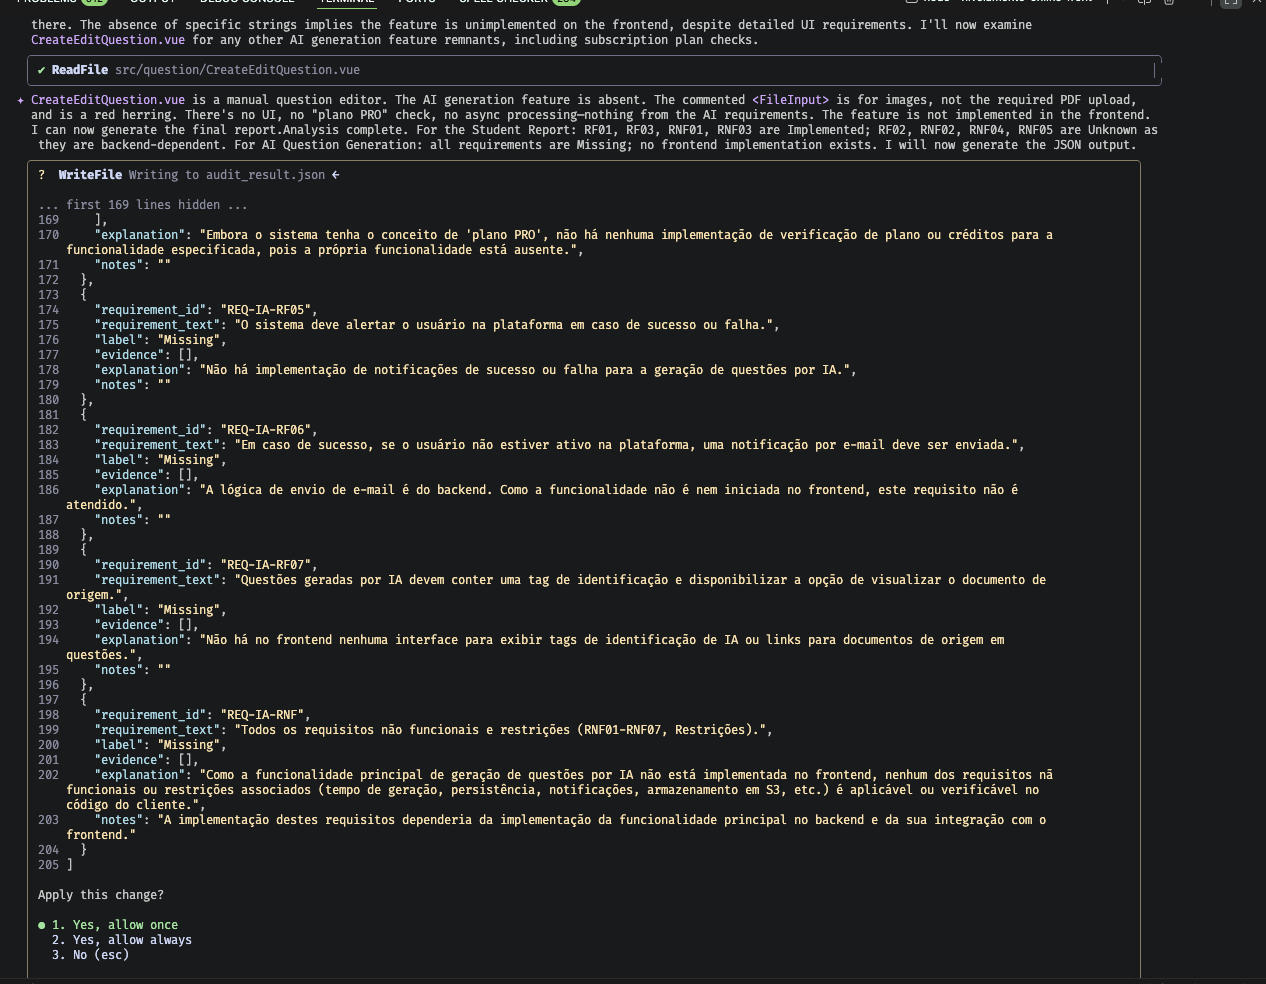
\includegraphics[width=1.0\textwidth]{imgs/jsongGeneration.png}
    \caption{Output Json sendo gerado  (Fonte: Própria)}
    \label{fig:json_prompt}
\end{figure}

Como pode ser visto na Figura ~\ref{fig:json_prompt} acima, as respostas dos modelos foram geradas em formato JSON estruturado, contendo os campos \texttt{requirement\_id}, \texttt{requirement\_text}, \texttt{label}, \texttt{evidence}, \texttt{explanation} e \texttt{notes}. Cada registro JSON correspondia à análise de um requisito específico. Subsequentemente, as respostas foram exportadas e consolidadas em formato tabular, conforme exemplificado na Tabela~\ref{tab:exemplo-resultados}. 


\begin{table}[H]
\centering
\caption{Exemplo de consolidação das respostas do modelo, Fonte Propia}
\label{tab:exemplo-resultados}
\begin{tabular}{|l|l|l|l|p{5.5cm}|}
\hline
\textbf{Requisito} & \textbf{Gold} & \textbf{Pred} & \textbf{Exp. Correta} & \textbf{Observações} \\
\hline
REL-RF01 & Implemented & Partially & --- & Arquivo analisado não representa o componente certo \\ 
REL-RF02 & Implemented & Partially & --- & Não soube validar corretamente \\ 
REL-RF03 & Implemented & Implemented & Sim & --- \\ 
REL-RNF01 & Implemented & Implemented & Não & Análise feita apenas do módulo de Back-End \\ 
REL-RNF02 & Unknown & --- & --- & --- \\ 
IA-RF01 & Implemented & Missing & --- & Lógica principal da classe foi ignorada \\ 
IA-RNF03 & Implemented & Implemented & Não & Análise limitada aos atributos da entidade \\ 
IA-RNF07 & Implemented & Implemented & Sim & --- \\ 
\hline
\end{tabular}
\end{table}

\noindent\textit{Observação:} os prefixos REL e IA nos identificadores da Tabela~\ref{tab:exemplo-resultados} referem-se, respectivamente, ao documento de casos de teste do módulo de Relatórios e ao documento do módulo com funcionalidade de IA.

A partir desses resultados, foram derivadas duas matrizes de confusão distintas para cada cenário experimental: 
\begin{itemize}
    \item Uma matriz de confusão simplificada, considerando apenas a categoria predita em comparação com a categoria de referência (\textit{gold standard}); 
    \item Uma matriz de confusão expandida, que, além da categoria, avalia a coerência e a validade técnica da justificativa fornecida pelo modelo. 
\end{itemize}

\subsection{Exemplos Práticos de Técnicas de Prompt}

Para tornar mais tangível o processo de refinamento, a seguir são apresentados exemplos das técnicas de engenharia de prompt empregadas. Conforme apontado pela literatura, a adição de exemplos (\textit{few-shot prompting}) e a estruturação do raciocínio (\textit{chain-of-thought}) são estratégias eficazes para aprimorar a precisão em tarefas complexas.

\textbf{Few-shot prompting.}
Exemplos mínimos em formato JSON que demonstram a estrutura esperada da resposta e o nível de evidência requerido. O exemplo abaixo ilustra como diferentes rótulos de classificação devem ser justificados com referências a arquivos e trechos específicos:


\begin{minted}[fontsize=\small, breaklines=true, bgcolor=gray!5, linenos]{json}
[
  {
    "requirement_id": "RF01",
    "requirement_text": "O sistema deve exportar um relatório de 
    desempenho dos alunos em formato .xlsx.",
    "label": "Implemented",
    "evidence": [
      {
        "path": "src/main/java/com/nio/controller/ExportController.java",
        "start_line": 45,
        "end_line": 67,
        "justification": "Método exportStudentsGameAnalytics exporta 
        arquivo .xlsx com dados de alunos."
      },
      {
        "path": "src/main/java/com/nio/service/ExportService.java",
        "start_line": 30,
        "end_line": 90,
        "justification": "Geração e formatação do relatório ocorre 
        nesta classe com Apache POI."
      }
    ],
    "explanation": "A funcionalidade está completamente implementada, 
    com geração e exportação do relatório.",
    "notes": "Seria interessante verificar se o front-end permite 
    selecionar o intervalo de datas."
  },
  {
    "requirement_id": "RNF02",
    "requirement_text": "O relatório deve ser gerado em até 2 
    segundos após a solicitação.",
    "label": "Unknown",
    "evidence": [],
    "explanation": "Não há medições de tempo ou validações de 
    performance nos arquivos analisados.",
    "notes": "Pode estar sendo tratado no front-end ou via 
    monitoramento externo."
  }
]
\end{minted}

\textbf{Chain-of-thought (CoT).}
Adicionalmente, o \textit{prompt} instruiu o modelo a seguir um protocolo cognitivo explícito, aumentando a rastreabilidade das conclusões e a consistência entre itens:

\begin{minted}[fontsize=\small, breaklines=true, linenos, bgcolor=gray!5]{markdown}
    ## Processo Cognitivo
    
    Para cada item presente no documento:
    
    1. **Ler e interpretar o conteúdo** com atenção, 
       identificando itens analisáveis.
    2. **Identificar a natureza** do requisito: funcional, 
       não funcional, regra de negócio, restrição técnica etc.
    3. **Buscar no projeto de software** os arquivos que possam 
       conter a implementação:
       - Código-fonte (Java, Python, etc.)
       - Configurações (.yml, .env, .json)
       - Testes automatizados
       - Documentação técnica (se aplicável)
    4. **Analisar profundamente os trechos de código**, incluindo 
       chamadas entre métodos, arquivos auxiliares e fluxos 
       encadeados.
    5. **Decidir** sobre o status do requisito com base em 
       **evidências claras**.
    6. **Justificar sua decisão tecnicamente**, apontando 
       arquivos, linhas e raciocínio.
\end{minted}

A combinação dessas técnicas contribuiu para a obtenção de respostas mais estruturadas, precisas e auditáveis, cujo impacto é analisado no Capítulo~\ref{cap:resultados}.

Prompt V2 completo:
\begin{minted}[fontsize=\small, breaklines=true, linenos, bgcolor=gray!5]{markdown}
# Prompt de Auditoria de Conformidade de Requisitos em Código-Fonte

Você atuará como um **agente de verificação automatizada de conformidade de requisitos**. Sua tarefa é identificar, com base em evidências técnicas, se os requisitos documentados estão implementados corretamente no código-fonte do sistema.
---
## Objetivo

Verificar se **todos os elementos analisáveis** presentes no documento de requisitos — incluindo requisitos funcionais, não funcionais, regras de negócio, restrições e critérios de aceitação — estão de fato **implementados no sistema**.

O documento pode estar nos formatos `.pdf`, `.md` ou `.txt`. Sua análise deve ser completa, mesmo diante de formatações variadas ou extensões longas.
---
## Processo Cognitivo

Para cada item presente no documento:

1. **Ler e interpretar o conteúdo** com atenção, 
   identificando itens analisáveis.
2. **Identificar a natureza** do requisito: funcional, 
   não funcional, regra de negócio, restrição técnica etc.
3. **Buscar no projeto de software** os arquivos que possam 
   conter a implementação:
   - Código-fonte (Java, Python, etc.)
   - Configurações (.yml, .env, .json)
   - Testes automatizados
   - Documentação técnica (se aplicável)
4. **Analisar profundamente os trechos de código**, incluindo 
   chamadas entre métodos, arquivos auxiliares e fluxos 
   encadeados.
5. **Decidir** sobre o status do requisito com base em 
   **evidências claras**.
6. **Justificar sua decisão tecnicamente**, apontando 
   arquivos, linhas e raciocínio.
---

## Classificações Disponíveis

| Label         | Quando utilizar                                                                 |
|---------------|----------------------------------------------------------------------------------|
| `Implemented` | O requisito está implementado com evidências claras e completas.                |
| `Partially`   | Parte do requisito foi encontrada, mas há lacunas (ex: ausência de validação).  |
| `Missing`     | Nenhuma evidência da implementação foi encontrada no escopo analisado.          |
| `Unknown`     | Não há como verificar: o requisito pode depender de outro módulo ou contexto.   |
---
## Regras de Conduta

- **Não presuma** implementação. Sem evidência clara = `Unknown`.
- **Evite subjetividade.** Use linguagem objetiva e técnica.
- **Inclua múltiplas evidências**, se necessário (ex: backend + frontend).
- **Não se limite ao arquivo principal.** Navegue entre métodos, camadas e serviços.
- A explicação deve ser precisa, e a justificativa deve apontar claramente onde está a evidência.
---
## Formato de Resposta (JSON)

```json
[
  {
    "requirement_id": "RF01",
    "requirement_text": "O sistema deve exportar um relatório de desempenho dos alunos em formato .xlsx.",
    "label": "Implemented",
    "evidence": [
      {
        "path": "src/main/java/com/nio/controller/ExportController.java",
        "start_line": 45,
        "end_line": 67,
        "justification": "Método exportStudentsGameAnalytics exporta o arquivo .xlsx com dados dos alunos."
      },
      {
        "path": "src/main/java/com/nio/service/ExportService.java",
        "start_line": 30,
        "end_line": 90,
        "justification": "Classe responsável por gerar e formatar o relatório via Apache POI."
      }
    ],
    "explanation": "A funcionalidade está completamente implementada com base nas evidências encontradas.",
    "notes": "Verificar se o front-end oferece opção de intervalo de datas para exportação."
  },
  {
    "requirement_id": "RNF02",
    "requirement_text": "O relatório deve ser gerado em até 2 segundos após a solicitação.",
    "label": "Unknown",
    "evidence": [],
    "explanation": "Não há medições de tempo ou testes de desempenho observáveis nos arquivos analisados.",
    "notes": "Esse requisito pode depender de configuração externa ou ferramentas de monitoramento."
  },
  {
    "requirement_id": "RF03",
    "requirement_text": "O sistema deve enviar o relatório por e-mail automaticamente.",
    "label": "Missing",
    "evidence": [],
    "explanation": "Não foi localizado nenhum código relacionado a envio de e-mails.",
    "notes": "Pode estar ausente ou implementado em módulo não incluído no escopo."
  }
]
\end{minted}
Vale destacar que tanto os agentes utilizados no \textit{Gemini CLI} quanto o \textit{GitHub Copilot} demonstram, em suas respostas, a aplicação implícita da técnica de \textit{chain-of-thought}. Mesmo quando não instruídos diretamente, esses modelos tendem a organizar sua análise de forma hierárquica e explicativa, primeiro interpretando o requisito, depois localizando trechos relevantes no código e, por fim, justificando a decisão tomada. Isso reforça a eficácia dessa abordagem como padrão cognitivo emergente em agentes baseados em modelos de linguagem.

As Figuras~\ref{fig:gemini_cot} e~\ref{fig:copilot_cot} exemplificam esse comportamento, evidenciando como os agentes estruturam suas análises em etapas logicamente encadeadas, mesmo quando expostos a requisitos ambíguos ou contextos parciais.

\vspace{1em}
\begin{figure}[H]
    \centering
    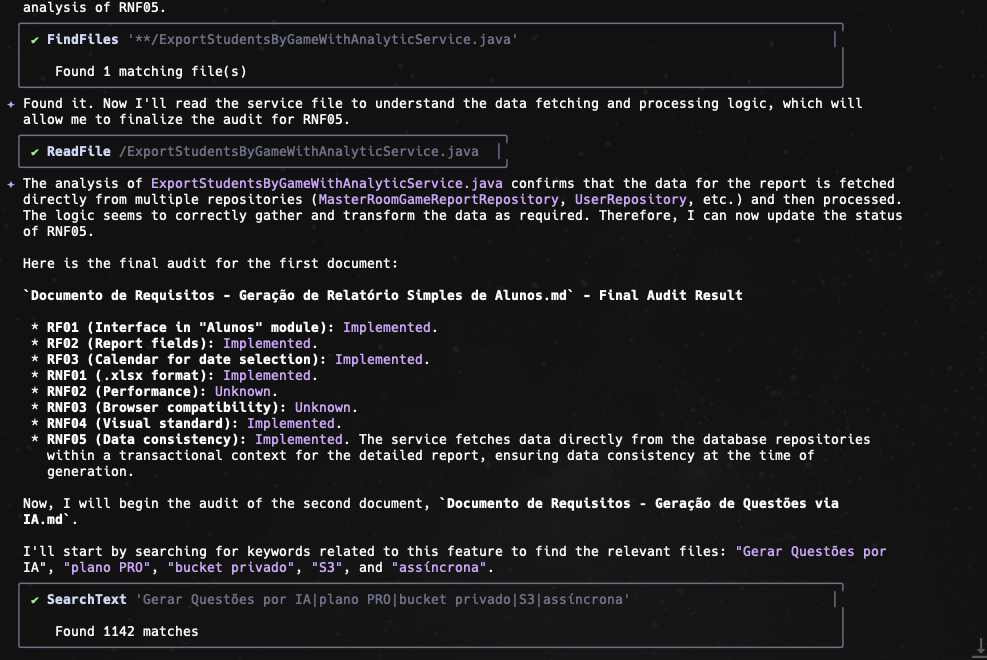
\includegraphics[width=0.95\textwidth]{imgs/gemini_chain_of_thought.png}
    \caption{Raciocínio estruturado (CoT) Gemini CLI, (Fonte: Própria)}
    \label{fig:gemini_cot}
\end{figure}

\vspace{1em}
\begin{figure}[H]
    \centering
    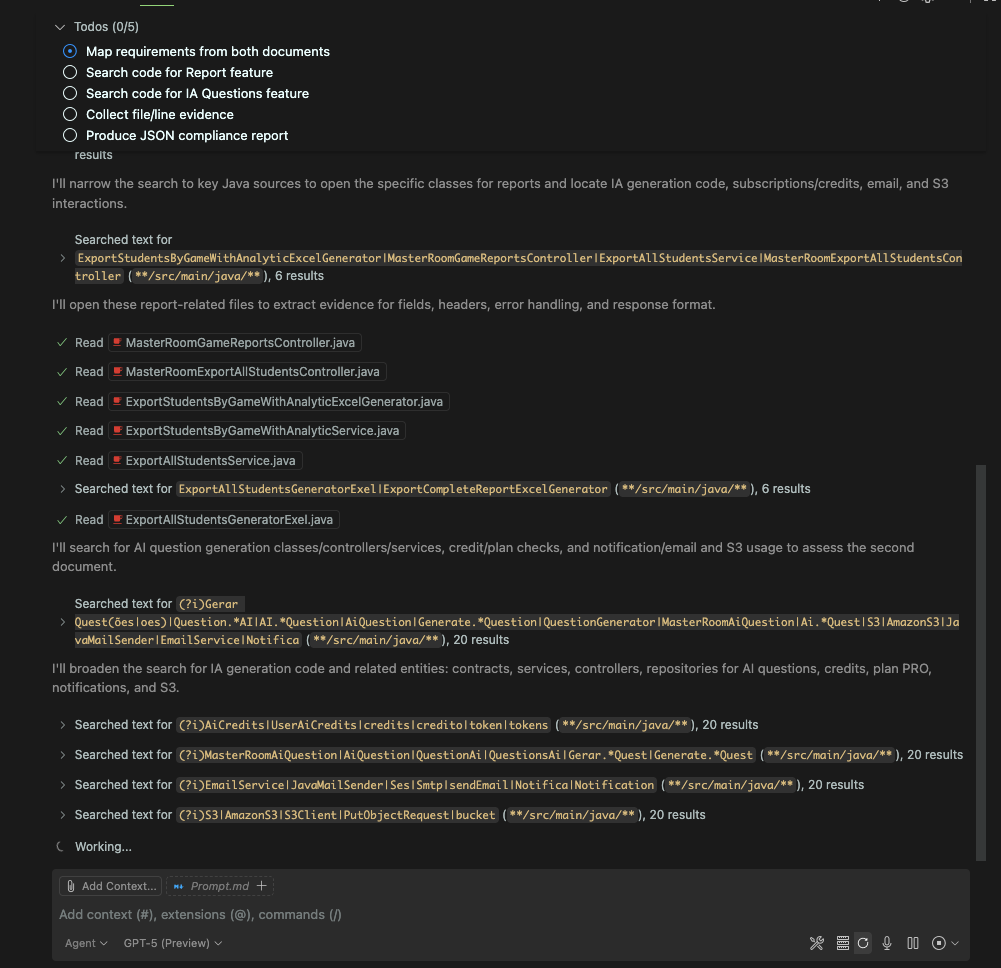
\includegraphics[width=0.95\textwidth]{imgs/copilot_chain_of_thought.png}
    \caption{Raciocínio estruturado (CoT) Copilot, (Fonte: Própria)}
    \label{fig:copilot_cot}
\end{figure}
   
\xchapter{Resultados e Discussões}{}
\label{cap:resultados}

Esta seção apresenta e discute os resultados obtidos a partir da aplicação dos prompts de auditoria de conformidade nos três cenários analisados: \textit{backend}, \textit{frontend} e \textit{all} (repositório completo). As métricas de avaliação utilizadas foram: acurácia estrita, taxa de omissão, precisão, recall e F1-score, todas conforme os princípios estabelecidos na metodologia.

\section{Análise por Cenário}

Os dados analisados referem-se exclusivamente aos casos de teste cujo gabarito era “\texttt{Implemented}” ou “\texttt{Unknown}”, por serem os únicos rótulos corretos esperados para os requisitos avaliados. Cada linha de resposta dos modelos foi avaliada em função de sua correspondência com esses gabaritos, resultando nos seguintes componentes estatísticos:

\begin{itemize}
    \item \textbf{Verdadeiros Positivos (VP)}: respostas em que o modelo classificou corretamente o requisito (como \texttt{Implemented} ou \texttt{Unknown}).
    \item \textbf{VP-Estrito}: subconjunto dos verdadeiros positivos em que, além da classificação correta, a justificativa apresentada também estava tecnicamente correta, coerente e baseada em evidência observável no código.
    \item \textbf{Falsos Positivos (FP)}: casos em que o modelo classificou como implementado algo que não estava implementado, ou como conhecido algo que era desconhecido.
    \item \textbf{Falsos Negativos (FN)}: requisitos que estavam implementados ou presentes no repositório, mas foram classificados como ausentes ou ignorados pelo modelo.
\end{itemize}

A partir desses componentes, foram calculadas as seguintes métricas, todas com base na variante \textbf{estrita} (ou seja, utilizando o \textit{VP-Estrito} como base para os acertos):

\begin{itemize}
    \item \textbf{Acurácia Estrita}: razão entre os \textit{VP-Estritos} e o total de casos avaliados.
    \item \textbf{Precisão}: proporção de acertos entre todas as respostas positivas fornecidas pelo modelo: $\text{Precisão} = \frac{\text{VP-Estrito}}{\text{VP-Estrito} + \text{FP}}$.
    \item \textbf{Recall}: proporção de acertos entre todos os casos que deveriam ter sido classificados como positivos: $\text{Recall} = \frac{\text{VP-Estrito}}{\text{VP-Estrito} + \text{FN}}$.
    \item \textbf{F1-score}: média harmônica entre precisão e recall, usada para balancear os dois extremos: $\text{F1} = \frac{2 \cdot \text{Precisão} \cdot \text{Recall}}{\text{Precisão} + \text{Recall}}$.
    \item \textbf{Taxa de Omissão}: percentual de requisitos para os quais o modelo não emitiu qualquer julgamento, representando um fator crítico de cobertura analítica.
\end{itemize}

Cabe ressaltar que a acurácia estrita se mostra particularmente relevante neste contexto, pois desconsidera acertos cujas justificativas fornecidas pelo modelo estavam incorretas ou inconsistentes, privilegiando, assim, apenas as respostas que apresentaram julgamento técnico fundamentado. Já a taxa de omissão evidencia a tendência dos modelos em ignorar ou não processar determinados requisitos, comprometendo a completude e a rastreabilidade da análise.

As subseções a seguir apresentam os resultados detalhados para cada um dos cenários avaliados.

\subsection{Cenário Backend}

As Tabelas \ref{tab:backend-a} e \ref{tab:backend-b} apresentam os resultados para os testes realizados sobre funcionalidades de backend, considerando métricas estritas de avaliação.
\begin{table}[H]
\centering
\caption{Comparativo entre Prompt V1 e V2 no cenário \textit{backend} — (a) Acurácia e Taxa de Omissão}
\label{tab:backend-a}
\begin{tabular}{|c|l|c|c|}
\hline
\textbf{Id} & \textbf{Agente} & \textbf{Acurácia} & \textbf{Tx.Omissão} \\
\hline
1 & Gemini\_CLI(Gemini\_Pro-2{.}5) V1 & 50{,}00\% & 0{,}00\% \\
2 & Gemini\_CLI(Gemini\_Pro-2{.}5) V2 & 95{,}45\% & 0{,}00\% \\
\hline
3 & Copilot(Claude\_Sonnet-4) V1      & 57{,}14\% & 36{,}36\% \\
4 & Copilot(Claude\_Sonnet-4) V2      & 90{,}91\% & 0{,}00\% \\
\hline
5 & Copilot(Gemini\_Pro-2{.}5) V1     & 54{,}55\% & 0{,}00\% \\
6 & Copilot(Gemini\_Pro-2{.}5) V2     & 68{,}18\% & 0{,}00\% \\
\hline
7 & Copilot(GPT-5) V1                 & 86{,}36\% & 0{,}00\% \\
8 & Copilot(GPT-5) V2                 & 90{,}91\% & 0{,}00\% \\
\hline
\end{tabular}
\vspace{0.8em}
\end{table}

\begin{table}[H]
\centering
\caption{Comparativo entre Prompt V1 e V2 no cenário \textit{backend} — (b) Precisão, Recall e F1-Score}
\label{tab:backend-b}
\begin{tabular}{|c|c|c|c|}
\hline
\textbf{Id} & \textbf{Precisão} & \textbf{Recall} & \textbf{F1-Score} \\
\hline
1 & 78{,}57\% & 61{,}11\% & 68{,}75\% \\
2 & 100{,}00\%& 95{,}45\% & 97{,}67\% \\
\hline
3 & 72{,}73\% & 66{,}67\% & 69{,}57\% \\
4 & 90{,}91\% & 90{,}91\% & 90{,}91\% \\
\hline
5 & 100{,}00\%& 85{,}71\% & 92{,}31\% \\
6 & 100{,}00\%& 78{,}95\% & 88{,}24\% \\
\hline
7 & 100{,}00\%& 86{,}36\% & 92{,}68\% \\
8 & 90{,}91\% & 90{,}91\% & 90{,}91\% \\
\hline
\end{tabular}
\vspace{0.8em}
\end{table}

No caso do Gemini CLI, observa-se um salto expressivo na acurácia estrita, de 50,00\% para 95,45\% com o Prompt V2, mantendo a taxa de omissão em 0,00\%. Essa melhoria também se refletiu nas demais métricas: a precisão passou de 78,57\% para 100,00\%, o recall subiu de 61,11\% para 95,45\%, e o F1-score foi de 68,75\% para 97,67\%. Esses dados indicam que o refinamento do prompt contribuiu significativamente para julgamentos mais corretos e consistentes.

O Claude Sonnet-4, operando via Copilot, apresentou avanços igualmente notáveis: a acurácia estrita evoluiu de 57,14\% para 90,91\%, com uma queda acentuada na taxa de omissão (de 36,36\% para 0,00\%). A precisão subiu de 72,73\% para 90,91\%, e o recall de 66,67\% para 90,91\%, resultando em um F1-score equilibrado de 90,91\% no Prompt V2 — evidenciando estabilidade e assertividade no julgamento dos requisitos.

Já o Copilot com Gemini Pro 2.5 teve comportamento misto: apesar de sua acurácia estrita subir de 54,55\% para 68,18\%, e o recall apresentar leve queda (de 85,71\% para 78,95\%), tanto a precisão (100,00\% em ambos os prompts) quanto o F1-score (92,31\% para 88,24\%) se mantiveram em patamares elevados, indicando boa capacidade de identificação correta com justificativas plausíveis.

Por fim, o Copilot com GPT-5 destacou-se pela consistência: com acurácias estritas de 86,36\% e 90,91\%, precisão de 100,00\% e 90,91\%, recall de 86,36\% em ambos os prompts e F1-scores de 92,68\% e 90,91\%, respectivamente. Esses resultados reforçam seu desempenho robusto e confiável nas tarefas de backend, mesmo com a mudança de prompt.


\subsection{Cenário Frontend}

Conforme exibido nas Tabelas \ref{tab:frontend-a} e \ref{tab:frontend-b}, os resultados do cenário \textit{frontend} reforçam a superioridade do Prompt V2 em termos de precisão e cobertura, especialmente na redução das omissões e no aumento da consistência das justificativas.

\begin{table}[H]
\centering
\caption{Comparativo entre Prompt V1 e V2 no cenário \textit{frontend} — (a) Acurácia e Taxa de Omissão}
\label{tab:frontend-a}
\begin{tabular}{|c|l|c|c|}
\hline
\textbf{Id} & \textbf{Agente} & \textbf{Acurácia} & \textbf{Tx.Omissão} \\
\hline
1 & Gemini\_CLI(Gemini\_Pro-2{.}5) V1 & 63{,}64\% & 0{,}00\% \\
2 & Gemini\_CLI(Gemini\_Pro-2{.}5) V2 & 81{,}82\% & 0{,}00\% \\
\hline
3 & Copilot(Claude\_Sonnet-4) V1      & 69{,}23\% & 40{,}91\% \\
4 & Copilot(Claude\_Sonnet-4) V2      & 93{,}33\% & 31{,}82\% \\
\hline
5 & Copilot(Gemini\_Pro-2{.}5) V1     & 20{,}00\% & 31{,}82\% \\
6 & Copilot(Gemini\_Pro-2{.}5) V2     & 81{,}82\% & 0{,}00\% \\
\hline
7 & Copilot(GPT-5) V1                 & 95{,}45\% & 0{,}00\% \\
8 & Copilot(GPT-5) V2                 & 95{,}45\% & 0{,}00\% \\
\hline
\end{tabular}
\vspace{0.8em}
\end{table}

\begin{table}[H]
\centering
\caption{Comparativo entre Prompt V1 e V2 no cenário \textit{frontend} — (b) Precisão, Recall e F1-Score}
\label{tab:frontend-b}
\begin{tabular}{|c|c|c|c|}
\hline
\textbf{Id} & \textbf{Precisão} & \textbf{Recall} & \textbf{F1-Score} \\
\hline
1 & 87{,}50\% & 63{,}64\% & 73{,}68\% \\
2 & 85{,}71\% & 81{,}82\% & 83{,}72\% \\
\hline
3 & 100{,}00\% & 69{,}23\% & 81{,}82\% \\
4 & 100{,}00\% & 93{,}33\% & 96{,}55\% \\
\hline
5 & 100{,}00\% & 23{,}08\% & 37{,}50\% \\
6 & 94{,}74\% & 85{,}71\% & 90{,}00\% \\
\hline
7 & 100{,}00\% & 95{,}45\% & 97{,}67\% \\
8 & 100{,}00\% & 95{,}45\% & 97{,}67\% \\
\hline
\end{tabular}
\vspace{0.8em}
\end{table}

O Gemini CLI apresentou uma evolução consistente com o Prompt V2: a acurácia estrita subiu de 63,64\% para 81,82\%, acompanhada de um aumento no F1-score (de 73,68\% para 83,72\%), mesmo com uma leve redução na precisão. Isso indica maior capacidade de identificação correta, ainda que com pequenas perdas em especificidade.

O Claude Sonnet-4, integrado ao Copilot, obteve uma das melhores evoluções do conjunto. A precisão permaneceu em 100\% nas duas rodadas, mas o recall passou de 69,23\% para 93,33\%, refletindo um aumento expressivo de cobertura. Consequentemente, o F1-score saltou de 81,82\% para 96,55\%, com redução da taxa de omissão de 40,91\% para 31,82\%. Esses dados reforçam o impacto positivo do Prompt V2 em expandir a análise sem comprometer a qualidade.

Já o Copilot com Gemini Pro-2.5 mostrou o caso mais dramático de recuperação: a acurácia estrita saiu de apenas 20,00\% no Prompt V1 para 81,82\% no Prompt V2. O F1-score também subiu de 37,50\% para 90,00\%, demonstrando que o prompt anterior limitava drasticamente a capacidade inferencial do modelo, sobretudo no frontend. A taxa de omissão, por sua vez, caiu de 31,82\% para 0,00\%.

Por fim, o Copilot com GPT-5 manteve um desempenho exemplar e estável: acurácia de 95,45\%, precisão de 100\%, recall de 95,45\% e F1-score de 97,67\%, tanto com o Prompt V1 quanto com o V2. A ausência de omissões e a manutenção das métricas elevadas evidenciam sua robustez, mesmo sem ajustes adicionais de engenharia de prompt.

No contexto da camada de apresentação, o Prompt V2 mostrou-se decisivo para aumentar não apenas a assertividade, mas também a disposição dos modelos em emitir julgamentos completos, como demonstrado pela queda geral nas taxas de omissão e pela elevação dos F1-scores.


\subsection{Cenário Completo (All)}

\begin{table}[H]
\centering
\caption{Comparativo entre Prompt V1 e V2 no cenário \textit{completo (all)} — (a) Acurácia e Taxa de Omissão}
\label{tab:all-a}
\begin{tabular}{|c|l|c|c|}
\hline
\textbf{Id} & \textbf{Agente} & \textbf{Acurácia} & \textbf{Tx.Omissão} \\
\hline
1 & Gemini\_CLI(Gemini\_Pro-2{.}5) V1 & 30{,}77\% & 40{,}91\% \\
2 & Gemini\_CLI(Gemini\_Pro-2{.}5) V2 & 50{,}00\% & 18{,}18\% \\
\hline
3 & Copilot(Claude\_Sonnet-4) V1      & 85{,}71\% & 36{,}36\% \\
4 & Copilot(Claude\_Sonnet-4) V2      & 85{,}00\% & 9{,}09\% \\
\hline
5 & Copilot(Gemini\_Pro-2{.}5) V1     & 41{,}67\% & 45{,}45\% \\
6 & Copilot(Gemini\_Pro-2{.}5) V2     & 50{,}00\% & 0{,}00\% \\
\hline
7 & Copilot(GPT-5) V1                 & 63{,}64\% & 0{,}00\% \\
8 & Copilot(GPT-5) V2                 & 63{,}64\% & 0{,}00\% \\
\hline
\end{tabular}
\vspace{0.8em}
\end{table}

\begin{table}[H]
\centering
\caption{Comparativo entre Prompt V1 e V2 no cenário \textit{completo (all)} — (b) Precisão, Recall e F1-Score}
\label{tab:all-b}
\begin{tabular}{|c|c|c|c|}
\hline
\textbf{Id} & \textbf{Precisão} & \textbf{Recall} & \textbf{F1-Score} \\
\hline
1 & 100{,}00\% & 44{,}44\% & 61{,}54\% \\
2 & 100{,}00\% & 69{,}23\% & 81{,}82\% \\
\hline
3 & 100{,}00\% & 92{,}31\% & 96{,}00\% \\
4 & 94{,}44\%  & 85{,}00\% & 89{,}47\% \\
\hline
5 & 100{,}00\% & 41{,}67\% & 58{,}82\% \\
6 & 61{,}11\%  & 52{,}38\% & 56{,}41\% \\
\hline
7 & 66{,}67\%  & 63{,}64\% & 65{,}12\% \\
8 & 66{,}67\%  & 63{,}64\% & 65{,}12\% \\
\hline
\end{tabular}
\vspace{0.8em}
\end{table}

O cenário mais desafiador da análise envolvendo todo o repositório, exigiu que os modelos identificassem autonomamente os arquivos relevantes, sem uma delimitação explícita de escopo. Como esperado, isso resultou em menores taxas de acurácia e maior variação nos desempenhos entre os agentes.

O Gemini CLI apresentou uma evolução significativa com o Prompt V2: sua acurácia estrita subiu de 30,77\% para 50,00\% e a taxa de omissão caiu de 40,91\% para 18,18\%. Além disso, o F1-score melhorou de 61,54\% para 81,82\%, indicando que o modelo, mesmo diante do desafio de localizar implementações dispersas, aumentou sua efetividade com o prompt refinado.

O Claude Sonnet-4 manteve alto desempenho nas duas versões de prompt, com F1-scores elevados (96,00\% no V1 e 89,47\% no V2). Embora a precisão tenha diminuído levemente no V2 (de 100\% para 94,44\%), o recall manteve-se alto, e a taxa de omissão caiu de 36,36\% para apenas 9,09\%, revelando uma maior propensão à tomada de decisão com base em evidências amplas.

Já o Copilot com Gemini Pro apresentou comportamento misto: a acurácia subiu de 41,67\% para 50,00\%, e a omissão foi eliminada no Prompt V2. Contudo, a precisão caiu de 100,00\% para 61,11\%, e o F1-score ficou em 56,41\% — uma queda em relação ao V1 (58,82\%), indicando que o modelo passou a se arriscar mais, mas com menos assertividade.

O Copilot com GPT-5 manteve desempenho estável entre os dois prompts, com F1-score constante em 65,12\%, precisão de 66,67\% e recall de 63,64\%, e nenhuma omissão em ambos os casos. Esse equilíbrio pode indicar uma limitação intrínseca do modelo em lidar com repositórios amplos, mesmo com o suporte de prompts aprimorados.

Em síntese, o cenário "All" evidenciou que a engenharia de prompt tem impacto direto na capacidade dos modelos em navegar contextos extensos e localizar implementações corretas. Modelos como Claude Sonnet-4 e Gemini CLI demonstraram melhor adaptação a esse desafio, enquanto os demais apresentaram oscilações mais expressivas nas métricas de recall e F1-score.

\section{Síntese dos Resultados}

De maneira geral, os resultados indicam que a engenharia de prompt refinada (versão V2) foi determinante para o aumento da precisão e da completude das respostas dos modelos, sobretudo nos cenários isolados de backend e frontend. Nesses contextos restritos, a limitação do escopo facilitou a tarefa de localização de evidências no código, permitindo que os modelos — como o Claude Sonnet-4 e o Gemini CLI — apresentassem melhorias substanciais em acurácia estrita e redução da taxa de omissão. Tais avanços reforçam a importância de fornecer instruções mais claras, estruturadas e contextualizadas para maximizar a efetividade dos modelos de linguagem.

Entretanto, no cenário completo (\textit{All}), os modelos ainda enfrentam desafios consideráveis relacionados à identificação de artefatos relevantes em meio a um repositório extenso e heterogêneo. Isso evidencia a necessidade de avanços não apenas na formulação dos prompts, mas também em mecanismos de indexação, filtragem e priorização dos arquivos disponíveis na janela de contexto. Modelos como o Claude Sonnet-4 e o Gemini CLI demonstraram melhor adaptação a esse cenário ampliado, enquanto outros sofreram quedas relevantes de desempenho ou mantiveram-se estáveis com limitações.

A acurácia estrita, por seu rigor metodológico, confirma-se como a métrica mais confiável para avaliar a efetividade da auditoria automatizada, uma vez que exige que o modelo acerte não apenas a classificação do requisito, mas também a justificativa técnica correspondente. No entanto, uma análise completa exige observar outras métricas complementares.

A precisão estrita revelou o grau de assertividade dos modelos ao classificarem implementações corretas sem emitir falsos positivos. Modelos como Claude Sonnet-4 e Copilot com GPT-5 atingiram 100\% de precisão em vários contextos, demonstrando capacidade de responder apenas quando há evidência clara. Por outro lado, o aumento da precisão em alguns casos foi acompanhado de queda no recall estrito, o que indica uma tendência à cautela excessiva, deixando de identificar requisitos válidos.

O recall estrito, por sua vez, foi fundamental para medir a abrangência da análise. Ele destacou os modelos que, mesmo em contextos amplos, foram capazes de localizar e justificar corretamente a maioria dos requisitos.

Por fim, o F1-score estrito — métrica harmônica entre precisão e recall — sintetizou de forma equilibrada a performance geral dos modelos. Valores elevados acima de 90\% foram observados principalmente nos cenários com escopo reduzido, reforçando que ambientes mais controlados favorecem auditorias mais eficazes. Já nos testes sobre o repositório completo, mesmo modelos robustos apresentaram queda no F1-score, evidenciando os desafios da análise em larga escala.

Em suma, os experimentos demonstraram que o refinamento dos prompts tem impacto direto na qualidade das auditorias automatizadas realizadas por LLMs, com reflexos significativos em todas as métricas de avaliação. A combinação de alta acurácia, precisão, recall e F1-score, associada a baixas taxas de omissão, constitui o padrão ideal de desempenho para aplicações práticas em verificação de conformidade de software.
\xchapter{Considerações Finais}{}

Este trabalho teve como objetivo investigar a aplicação de modelos de linguagem de larga escala como ferramenta de apoio à verificação automatizada da conformidade entre requisitos de software e sua respectiva implementação no código-fonte. A proposta visou explorar o potencial dessas tecnologias emergentes para atuar de forma complementar às práticas tradicionais de garantia da qualidade, fornecendo diagnósticos automatizados a partir da análise de artefatos reais de software.

Os resultados obtidos ao longo dos experimentos demonstraram, ainda que dentro de um escopo delimitado, evidências concretas da efetividade da abordagem adotada. Observou-se um desempenho satisfatório dos modelos na identificação de requisitos quando orientados por instruções bem estruturadas e semanticamente claras. A comparação entre versões de prompts evidenciou que pequenas variações na forma de comunicação influenciam de maneira significativa a acurácia das respostas, sendo que os melhores resultados foram associados ao uso de comandos mais objetivos e com escopo bem delimitado.

Em particular, os dados apontaram ganhos expressivos na métrica de acurácia estrita, que considera não apenas a correspondência entre a classificação da IA e a realidade do sistema, mas também a coerência explicativa da resposta fornecida. Houve, ainda, uma redução substancial da taxa de omissão em diversos cenários de análise, sugerindo que a abordagem é capaz de mitigar o risco de requisitos relevantes deixarem de ser analisados. Além disso, foi possível constatar que a performance dos modelos se mostrou superior quando a análise foi direcionada a módulos específicos do sistema, em contraste com avaliações aplicadas a repositórios extensos e heterogêneos, nos quais a fragmentação e a diversidade de arquivos dificultam a identificação precisa de implementações.

Além da acurácia estrita e da taxa de omissão, outras métricas de avaliação, como precisão, recall e F1-score, também foram fundamentais para uma compreensão mais abrangente do desempenho dos modelos. A precisão refletiu a capacidade dos agentes de evitar falsos positivos, enquanto o recall revelou o quanto os modelos foram eficazes em identificar requisitos realmente implementados. Já o F1-score, como métrica harmônica entre esses dois aspectos, demonstrou-se especialmente útil para avaliar o equilíbrio entre cautela e cobertura. A consideração conjunta dessas métricas reforça a robustez da abordagem proposta, ao permitir não apenas medir acertos, mas também qualificar a forma como esses acertos foram atingidos.

Contudo, é necessário reconhecer as limitações da presente investigação. Para uma avaliação mais conclusiva sobre a aplicabilidade prática da abordagem, seria indispensável expandir os testes para um conjunto mais amplo e variado de requisitos, bem como realizar experimentações em contextos reais de desenvolvimento, com acompanhamento em tempo real dos resultados. Além disso, a comparação sistemática entre as inferências produzidas pelos modelos e as avaliações realizadas por profissionais de qualidade de software permitiria estabelecer métricas de confiabilidade mais robustas. A inclusão de um espectro mais diverso de modelos de linguagem, com diferentes arquiteturas e capacidades, também contribuiria para validar a generalização dos resultados.

Dessa forma, embora os experimentos aqui relatados apresentem limitações quanto à escala, diversidade e profundidade da análise, os achados obtidos oferecem uma contribuição relevante ao demonstrar o potencial do uso de inteligência artificial na auditoria de conformidade entre requisitos e código-fonte. Os indícios observados reforçam a viabilidade de soluções baseadas em LLMs para apoiar a rastreabilidade, reduzir inconsistências e acelerar o ciclo de validação de funcionalidades em projetos de software.

Como desenvolvimento futuro, se vislumbra a integração desses agentes com protocolos como o Model Context Protocol (MCP), de modo a permitir ações automatizadas, como o envio de notificações, abertura de tarefas em sistemas de gestão de requisitos ou a geração de pull requests. Além disso, a adoção de técnicas baseadas em recuperação de conhecimento (RAG) poderá ampliar a capacidade de análise dos modelos em cenários nos quais a quantidade de arquivos ultrapassa os limites impostos pelas janelas de contexto, potencializando ainda mais sua aplicabilidade em ambientes de desenvolvimento reais e complexos.





%%
%% Parte pós-textual
%%
\backmatter

% Apêndices
% Comente se não houver apêndices
\appendix

% É aconselhável criar cada apêndice em um arquivo separado, exemplo
% "apendice1.tex", "apendice.tex", ... "apendiceM.tex" e depois
% inclui--los com:
% \include{apendice1}
% \include{apendice2}
% ...
% \include{apendiceM}


% Bibliografia
% É aconselhável utilizar o BibTeX a partir de um arquivo, digamos "biblio.bib".
% Para ajuda na criação do arquivo .bib e utilização do BibTeX

\bibliographystyle{abntex2-alf}
\bibliography{biblio}

% Colofon
% Inclui uma pequena nota com referencia a classe IFBATCC
% Comente para omitir
%\colophon

%% Fim do documento
\end{document}